\documentclass[10pt]{beamer}
\mode<presentation>
\usetheme{Warsaw}
%\usetheme{Madrid}
\usecolortheme{orchid}
\transdissolve[duration=0.2]
\setbeamertemplate{headline}{}
\beamertemplatenavigationsymbolsempty

\usefonttheme{serif}
\usepackage{sans}
\usepackage{rotating}
\usepackage{xcolor}

\usepackage{listings}
\lstset{language=C++,
  basicstyle=\scriptsize\ttfamily,
  keywordstyle=\color{blue}\ttfamily,
  stringstyle=\color{red}\ttfamily,
  commentstyle=\color{green}\ttfamily,
  morecomment=[l][\color{magenta}]{\#},
  xleftmargin=2em,
%  frame=single,
  frame=lines,
  framexleftmargin=0em,
  numbers=left,
  escapeinside={(*@}{@*)}%  escapechar=|
}
\usepackage{epsfig}
\usepackage{amsmath}
\usepackage{amssymb}
\usepackage{ifthen}
\usepackage{color}
\usepackage{boxedminipage}
\usepackage{colortbl}
\usepackage{array}
\usepackage{soul}
\makeatletter
\newcommand\SoulColor{%
  \let\set@color\beamerorig@set@color
  \let\reset@color\beamerorig@reset@color}
\makeatother
\usepackage{graphics}
\usepackage{moreverb}
\usepackage{rotating}
\usepackage{psfrag}
\usepackage{subfigure}
\usepackage{url}
\usepackage{graphicx}
\usepackage{graphics}
\usepackage{rotating}
\usepackage{multirow}
\usepackage{url}
\usepackage{amsfonts}
\usepackage{balance}
\usepackage{tikz}
\usetikzlibrary{decorations,arrows,shapes}

\definecolor{dodgerblue}{rgb} {0.4,0.4,1.0} % azul
\definecolor{forestgreen}{rgb}{1.0,0.0,0.0} % rojo
\definecolor{yellow1}{rgb}    {0.0,1.0,0.0} % verde

\definecolor{darkred}{rgb}{0.44,0,0}
\definecolor{darkgreen}{rgb}{0,0.44,0}
\definecolor{darkblue}{rgb}{0,0,0.44}
\definecolor{grey}{rgb}{0.5,0.5,0.5}

\definecolor{lightgreen}{RGB} {1,204,204} % magenta
\definecolor{pink}{RGB}       {254,152,254} % magenta

\newcommand{\sytrd}{\mbox{\sc sytrd}} 
\newcommand{\syrdb}{\mbox{\sc syrdb}} 
\newcommand{\sbrdb}{\mbox{\sc sbrdb}} 
\newcommand{\sbrdt}{\mbox{\sc sbrdt}} 
\newcommand{\symm}{\mbox{\sc  symm}} 
\newcommand{\hemm}{\mbox{\sc  hemm}} 
\newcommand{\syrtk}{\mbox{\sc syr2k}} 
\newcommand{\hertk}{\mbox{\sc her2k}} 
\newcommand{\syrt}{\mbox{\sc syr2}} 
\newcommand{\syrk}{\mbox{\sc syrk}} 
\newcommand{\herk}{\mbox{\sc herk}} 
\newcommand{\gemm}{\mbox{\sc  gemm}} 
\newcommand{\gebp}{\mbox{\sc  gebp}} 
\newcommand{\gepp}{\mbox{\sc  gepp}} 
\newcommand{\trsm}{\mbox{\sc  trsm}} 
\newcommand{\trmm}{\mbox{\sc  trmm}} 
\newcommand{\symv}{\mbox{\sc  symv}} 
\newcommand{\gemv}{\mbox{\sc  gemv}} 
\newcommand{\ger} {\mbox{\sc  ger}} 
\newcommand{\scal}{\mbox{\sc scal}}
\newcommand{\chol}{\mbox{\sc  chol}} 

\newcommand{\libflame}[0]{{\tt libflame}}
\newcommand{\striu}{{\rm striu}}
\newcommand{\half}{\frac{1}{2}}
\newcommand{\sign}{\mbox{sign}}
\newtheorem{algorithm}{Algorithm}
\newcommand{\hous}{{\rm Hous}}
\newcommand{\trilu}[1]{\mbox{\sc trilu}(#1)}

\usepackage{algorithmic}
\usepackage{algorithm}
\usepackage{multirow}
\usepackage{colortbl}
\usepackage{float}

\usepackage[utf8]{inputenc}
\usepackage[spanish]{babel}

\usepackage{epstopdf}

\setbeamercovered{transparent} 
\setbeamercolor{background canvas}{bg=white}

\defbeamertemplate*{footline}{shadow theme}{%
\leavevmode%
\hbox{\begin{beamercolorbox}[wd=.5\paperwidth,ht=2.5ex,dp=1.125ex,leftskip=.3cm plus1fil,rightskip=.3cm]{author in head/foot}%
    \usebeamerfont{author in head/foot}\hfill\insertshortauthor
\end{beamercolorbox}%

\begin{beamercolorbox}[wd=.5\paperwidth,ht=2.5ex,dp=1.125ex,leftskip=.3cm,rightskip=.3cm plus1fil]{title in head/foot}%
    \usebeamerfont{title in head/foot}\insertshorttitle\hfill%
\insertframenumber\,/\,\inserttotalframenumber
\end{beamercolorbox}}%
\vskip0pt%
}


\title[]{\large
  Evaluación y optimización de rendimiento y consumo energético de
  aplicaciones paralelas a nivel de tareas sobre arquitecturas asimétricas}

\date{}

\author[]{
  \scriptsize Luis Mª Costero\\[0.6cm]
  \scalebox{0.25}{\includegraphics[]{logos/Negro-transparente}}\\[-0.3cm]
}

\AtBeginSection[] {
  \begin{frame}
    \frametitle{Índice}
    \tableofcontents[currentsection]
  \end{frame}
}

\begin{document}
\frame[plain]{\vspace{0.6cm} \centering
  
  \hspace{0.1cm}
  \begin{minipage}{0.85\textwidth}
    \centering
    % \scriptsize \textsc{Máster en Ingeniería Informática\\ \medskip
    %   Madrid, 20 de septiembre de 2016}
    \small \textsc{Máster en Ingeniería Informática}\\ \medskip
    \small \textsc{Trabajo fin de Máster} \\ \medskip
    \scriptsize \textsc{20 de septiembre de 2016}
  \end{minipage}\\[0.70cm]
  \small
  \scriptsize
  \titlepage
}

%===========================================================================
\begin{frame}
  \frametitle{Índice}
  \tableofcontents
\end{frame}

%===========================================================================
\section{Arquitecturas asimétricas}

\begin{frame}
  \frametitle{Introducción}

  \vfill

  \begin{columns}
    \begin{column}{0.5\textwidth}
      \begin{center}
        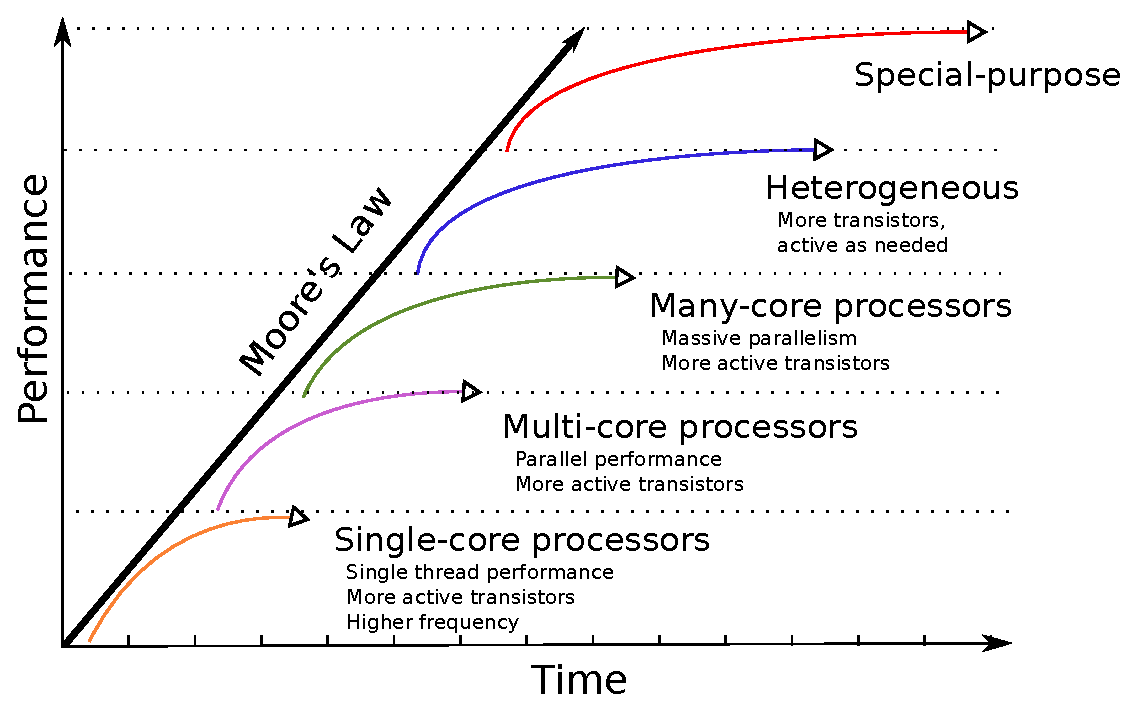
\includegraphics[width=1.0\textwidth]{Figures/hofstee.eps}
      \end{center}      
    \end{column}
    \begin{column}{0.5\textwidth}
      \begin{block}{Tendencia actual}
        \begin{center}
          Heterogeneidad + especialización
        \end{center}
      \end{block}      
    \end{column}
  \end{columns}

  \vfill

  \begin{exampleblock}{Nueva tendencia: {\bf procesadores asimétricos} de bajo consumo}
    \begin{itemize}
    \item ¿Válidos para propósito general en HPC?
    \item ¿Cómo explotar la asimetría eficientemente?
    \item ¿Cómo aprovechar los planificadores de tareas actuales?
    \end{itemize}
  \end{exampleblock}

\end{frame}



% \begin{frame}
%   \frametitle{Introducción}
  
%   Present and future of High Performance Computing: 
  
%   \vfill
  
%   \begin{itemize}
    
%   \item Technological advance $\Rightarrow$ performance improvement.
    
%     \begin{itemize}
%       \scriptsize
%       % \item Processors works at higher frequencies
%     \item Higher number of cores per socket (processor)
%     \item Hardware accelerators to boost performance (GPU/multi-GPU, Xeon Phi\ldots) 
%     \end{itemize}
    
%     \vfill
    
%   \item Common trend: more cores, accelerators $\Rightarrow$ \textcolor{darkred}{Higher energy consumption}
    
%     \vfill
    
%   \item New trend: Low-power processors $\Rightarrow$ \textcolor{darkgreen}{Higher energy efficiency}
    
%     \vfill
    
%   \item Newer trend: {\bf Asymmetric} low-power processors $\Rightarrow$ \textcolor{darkblue}{Task adaptation}
%     \begin{itemize}
%     \item Valid/useful for general-purpose HPC?
%     \item How to efficiently exploit asymmetry in architectures? 
%     \item How to leverage existing task schedulers to exploit asymmetry?
%     \end{itemize}
%   \end{itemize}
% \end{frame}




\begin{frame} %----
  \frametitle{Arquitecturas asimétricas}
  
  {\bf Arquitecturas asimétricas (AMPs):}
  \vspace{1cm}
  \begin{columns}[onlytextwidth]
    \begin{column}{0.2\textwidth}
      \centering
      \fboxsep=2.5mm \fboxrule=.5mm
      \fcolorbox{black}{blue!50!white}{\small BIG0}
      
      \fcolorbox{black}{blue!50!white}{\small BIG1}
      
      % \fcolorbox{black}{blue!50!white}{\footnotesize BIG2}
      
      % \fcolorbox{black}{blue!50!white}{\footnotesize BIG3}
      
      \fboxsep=1.5mm \fboxrule=.5mm
      \fcolorbox{black}{blue!10!white}{\scriptsize LITTLE0}
      
      \fcolorbox{black}{blue!10!white}{\scriptsize LITTLE1}
      
      \fcolorbox{black}{blue!10!white}{\scriptsize LITTLE2}
      
      \fcolorbox{black}{blue!10!white}{\scriptsize LITTLE3}
    \end{column}
    
    \begin{column}{0.8\textwidth}    
      \begin{itemize}
        \small
      \item Formadas por dos tipos de procesadores:
        \begin{itemize}
          \small
        \item {\bf big}: alto rendimiento, alto consumo energético.
        \item {\bf LITTLE}: bajo rendimiento, bajo consumo energético.
        \end{itemize}
        
      \item Conjunto de instrucciones común. Compatibilidad binaria.  
      \item Transparente para el usuario (a través de soporte del SO).
      \item Ejemplos: ARM big.LITTLE, Intel QuickIA, SMPs con núcleos
        ejecutando a diferentes frecuencias, \ldots
      \end{itemize}
    \end{column}
  \end{columns} 
\end{frame}

\begin{frame}
  \frametitle{Arquitecturas ARM big.LITTLE}
  \only<1>
  { 
    {\bf Plataformas utilizadas:}

    \vfill
    \begin{columns}[onlytextwidth]
      \begin{column}{0.5\textwidth}
        \includegraphics[width=0.9\textwidth]{Figures/Exynos-2.pdf}
        
        \footnotesize
        {\bf Hardkernel ODROID XU3}
        \begin{itemize}
        \item {\sc big:} 4 Cortex-A15 (1.3 GHz)
        \item {\sc LITTLE:} 4 Cortex-A7 (1.3 GHz)
        \item Medidores consumo integrados. 
        \end{itemize}
      \end{column}
      
      \begin{column}{0.5\textwidth}
        \includegraphics[width=0.9\textwidth]{Figures/Juno.pdf}
        
        {
          \footnotesize
          {\bf ARM Juno board}
          \begin{itemize}
          \item {\sc big:} 2 Cortex A57 (1.1 GHz)
          \item {\sc LITTLE:} 4 Cortex A53 (850 MHz)
          \item Resistencias de {\em shunt}.
          \end{itemize}
        }
      \end{column}
    \end{columns}
  }
\end{frame}

%===========================================================================
\section{Estrategias para la extracción de paralelismo en AMPs}
\begin{frame}
  \frametitle{Soluciones Software para explotar la asimetría}
  
  \begin{columns}[onlytextwidth]
    \begin{column}{0.6\textwidth}
      \centering
      \fboxsep=4mm \fboxrule=1mm
      \fcolorbox{black}{blue!50!white}{Biblioteca}
      
      $\uparrow$
      
      \fcolorbox{black}{blue!30!white}{Planificador de tareas}
      
      $\uparrow$
      
      \fcolorbox{black}{blue!10!white}{OS}
    \end{column}
    
%    \begin{column}{0.\textwidth}
%    \end{column}
    
    \begin{column}{0.4\textwidth}
      \footnotesize
      \begin{itemize}
      \item Ej. Biblioteca BLIS.
%      \item Pros: Específica para una aplicación y arquitectura concreta.
%      \item Cons: Implementación específica para la arquitectura. 
      \end{itemize}
      
      \vspace{0.3cm}
      \hrulefill
      \vspace{0.3cm}
      
      \begin{itemize}
      \item Ej. OmpSs / Nanox.
%      \item Pros: Facilidad de programar, en general.
%      \item Cons: Políticas de planificación complejas.
      \end{itemize}
      
      \vspace{0.3cm}
      \hrulefill
      \vspace{0.3cm}
      
      \begin{itemize}
      \item Ej. Planificador Linux.
%      \item Pros: General, completamente transparente para las aplicaciones.
%      \item Cons: Rendimiento?
      \end{itemize}
      \vfill
    \end{column}
  \end{columns}
  
  \vfill
  
  \begin{itemize}
  \item La asimetría de la arquitectura puede ser tratada en diferentes
    niveles del Software.    
  \item Solución de compromiso entre la facilidad de programación,
    generalidad, rendimiento \ldots    
  \end{itemize}  
\end{frame}


\begin{frame}
  \frametitle{Extracción del paralelismo en AMPs: Sistema Operativo}

  \begin{figure}%[tbh!]
    \centering
    \subfigure[Clustered]{
      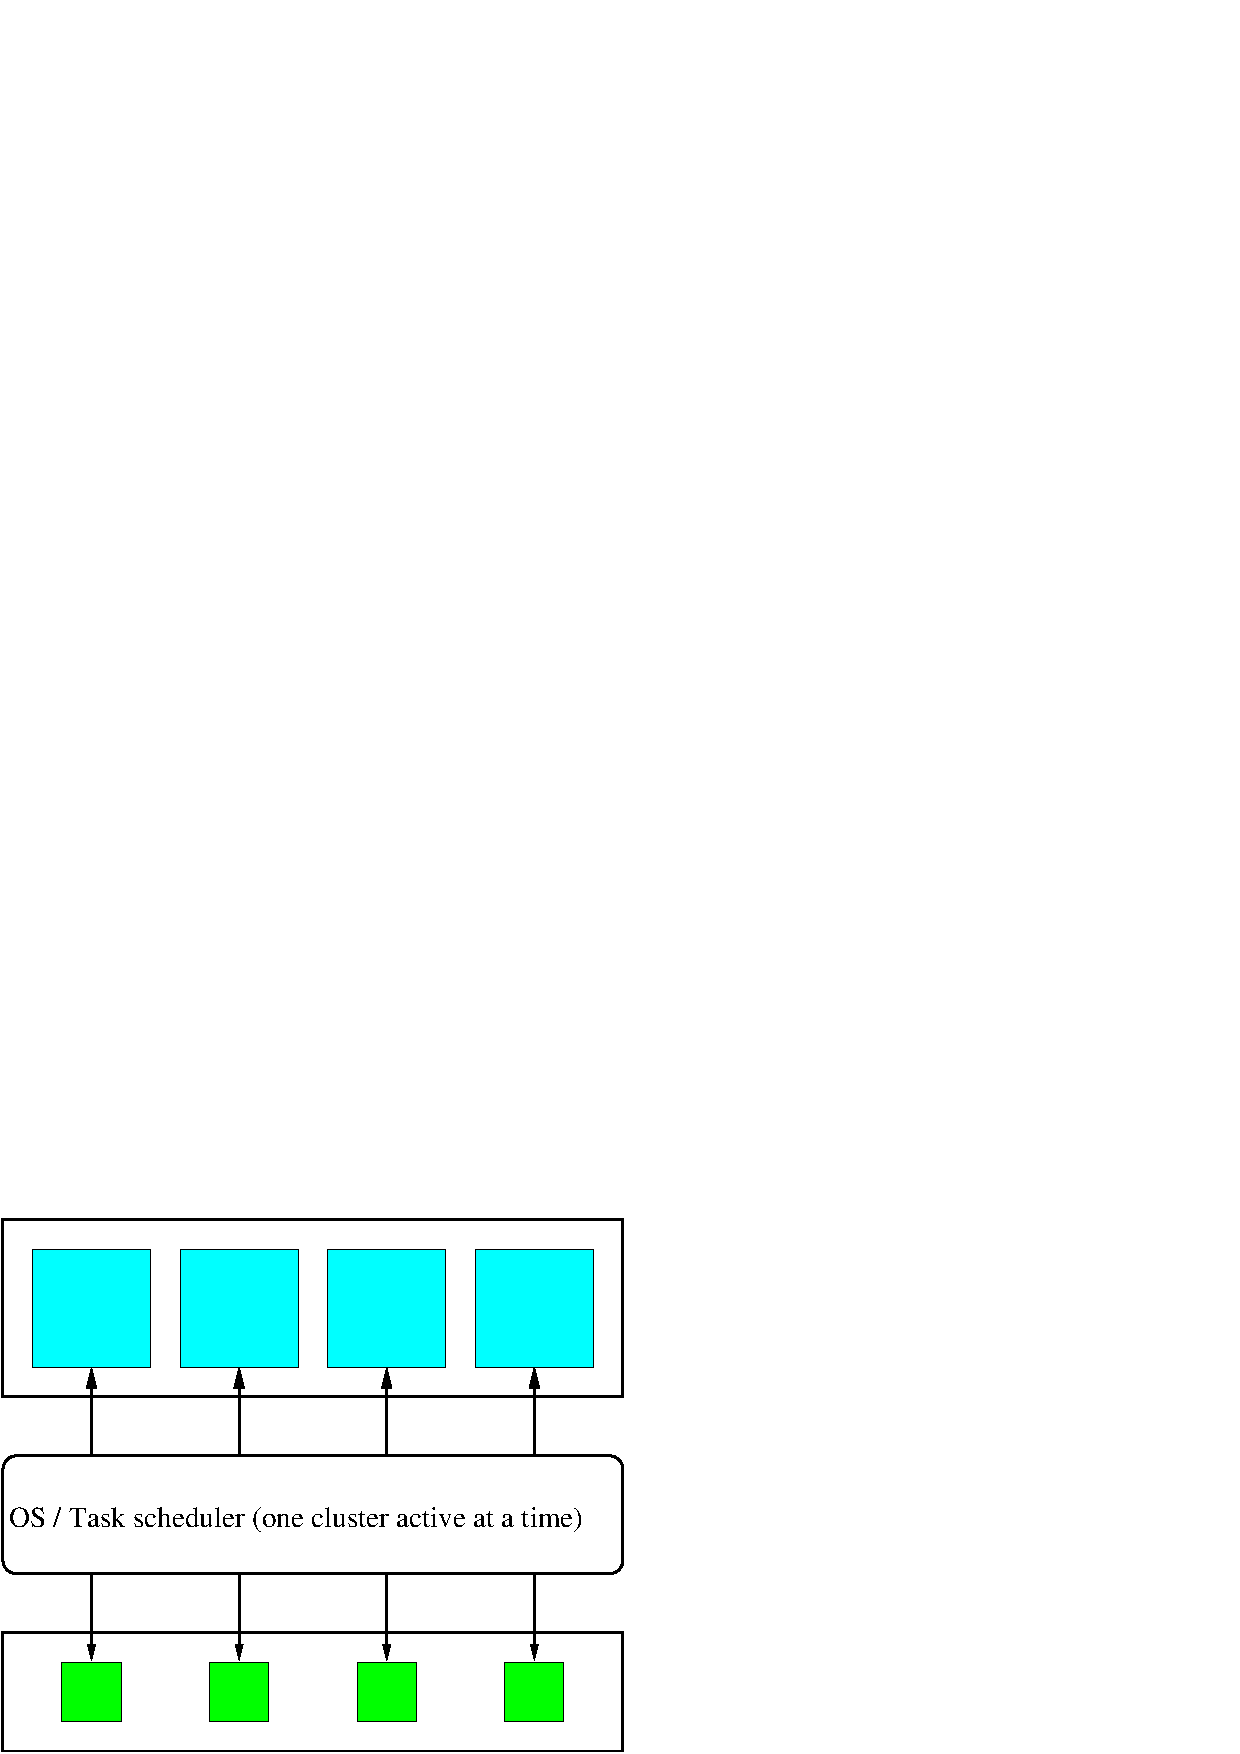
\includegraphics[width=0.3\textwidth]{Figures/clustered.pdf}
    }
    \subfigure[IKS]{
      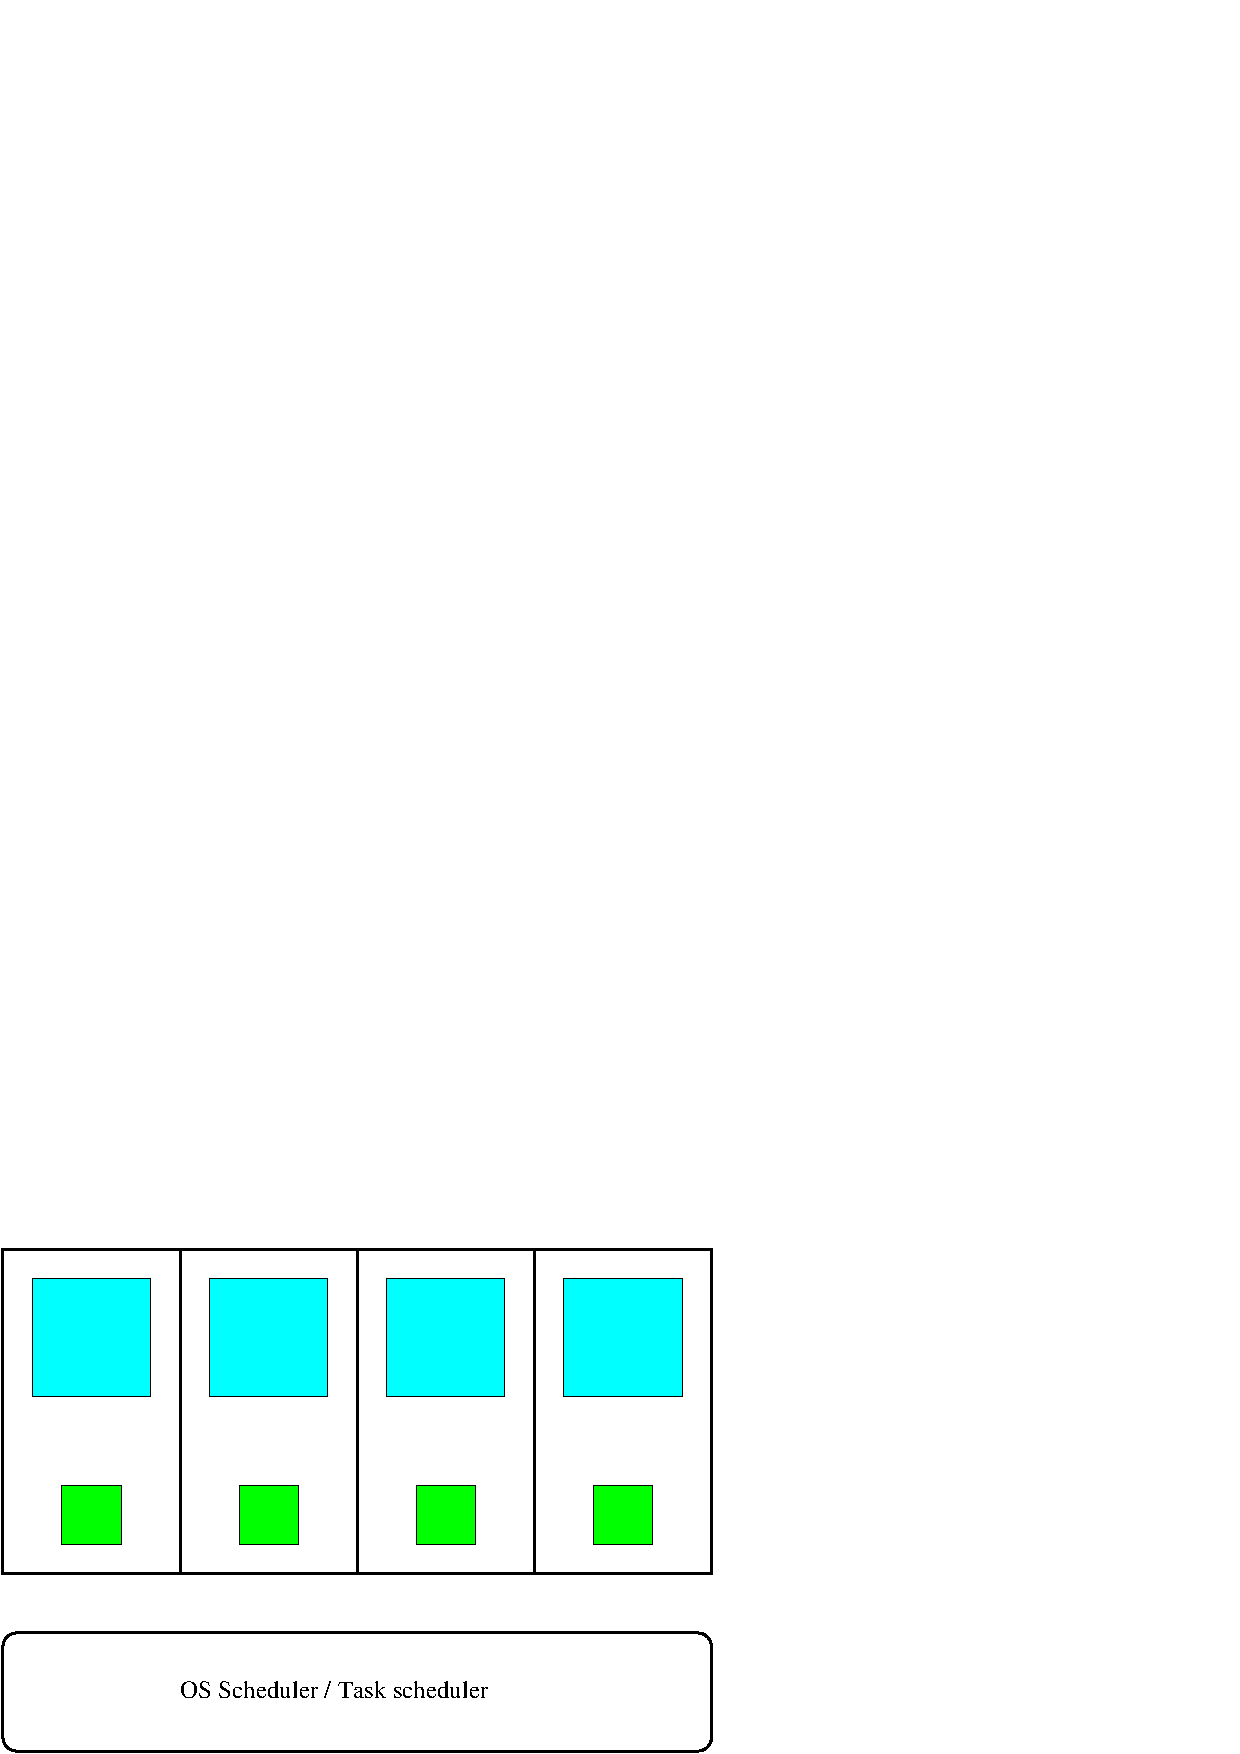
\includegraphics[width=0.3\textwidth]{Figures/iks.pdf}
    }
    \subfigure[GTS]{
      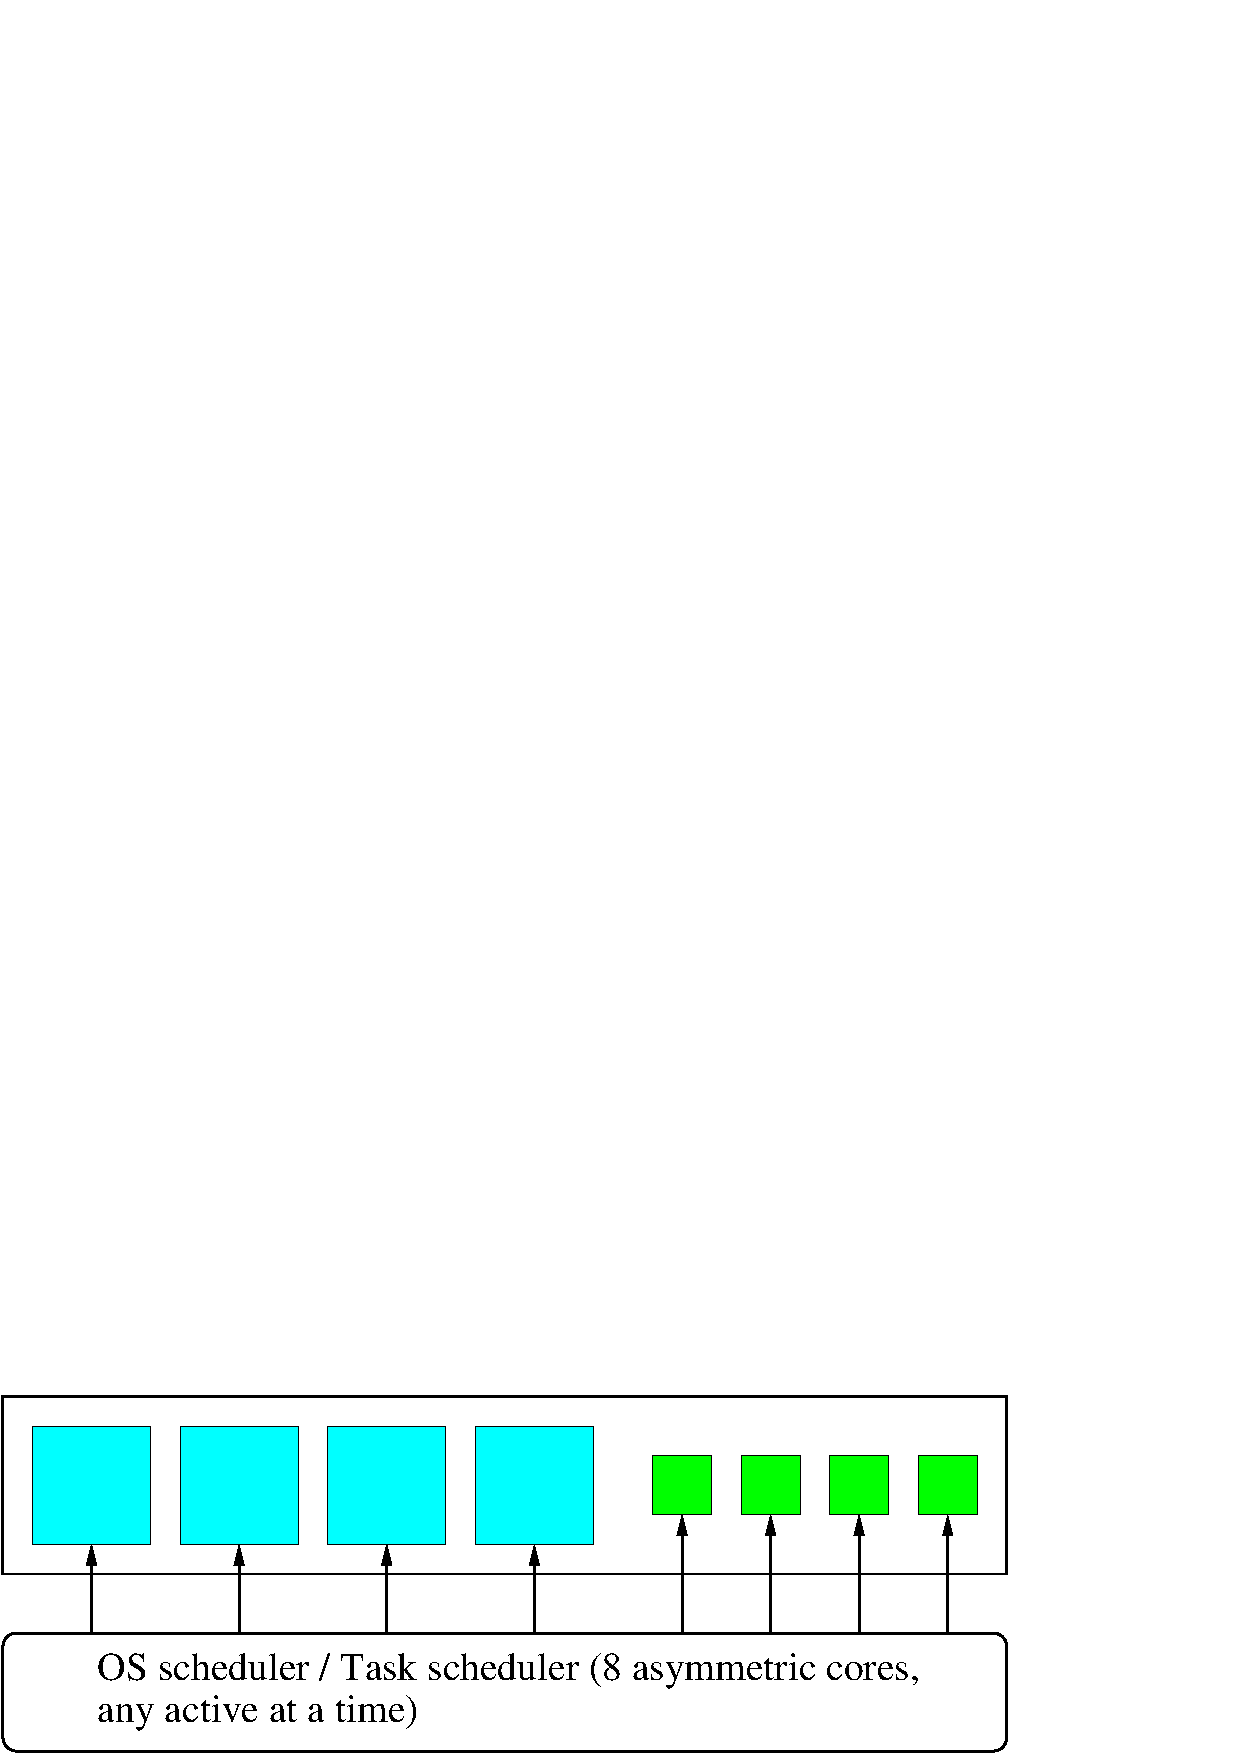
\includegraphics[width=0.3\textwidth]{Figures/gts.pdf}
    }
    \caption{Modos de funcionamiento para arquitecturas big.LITTLE en Linux.}
    \label{fig:modes}
  \end{figure}

  
  \begin{itemize}
  \item {\bf Ventajas:} General, totalmente transparente al usuario.
  \item {\bf Inconvenientes:} ¿Rendimiento?
  \end{itemize}
\end{frame}


\begin{frame}[fragile]
  \frametitle{Extracción del paralelismo en AMPs: Planificador de tareas}
  \begin{columns}
    \begin{column}{0.9\textwidth}
\begin{lstlisting}[language=C++]
(*@\SoulColor\hl{\#pragma omp task inout([b][b]A)}@*)
void po_cholesky (double *A, int b, int ld){

 static int        INFO = 0;
 static const char UP   = 'U';
 dpotrf (&UP, &b, A, &ld, &INFO);
}

(*@\SoulColor\hl{\#pragma omp task in([b][b]A) inout([b][b]B)} @*)
void tr_solve (double *A, double *B, int b, int ld){

 static double     DONE = 1.0;
 static const char LE   = 'L', UP = 'U', TR = 'T', NU = 'N';
 dtrsm (&LE, &UP, &TR, &NU, &b, &b, &DONE, A, &ld, B, &ld);
}
\end{lstlisting}
    \end{column}
    \begin{column}{0.1\textwidth}
      \rotatebox{90}{Programador}
    \end{column}

  \end{columns}


 \begin{columns}[c]%[onlytextwidth]
    \begin{column}{0.20\textwidth}
      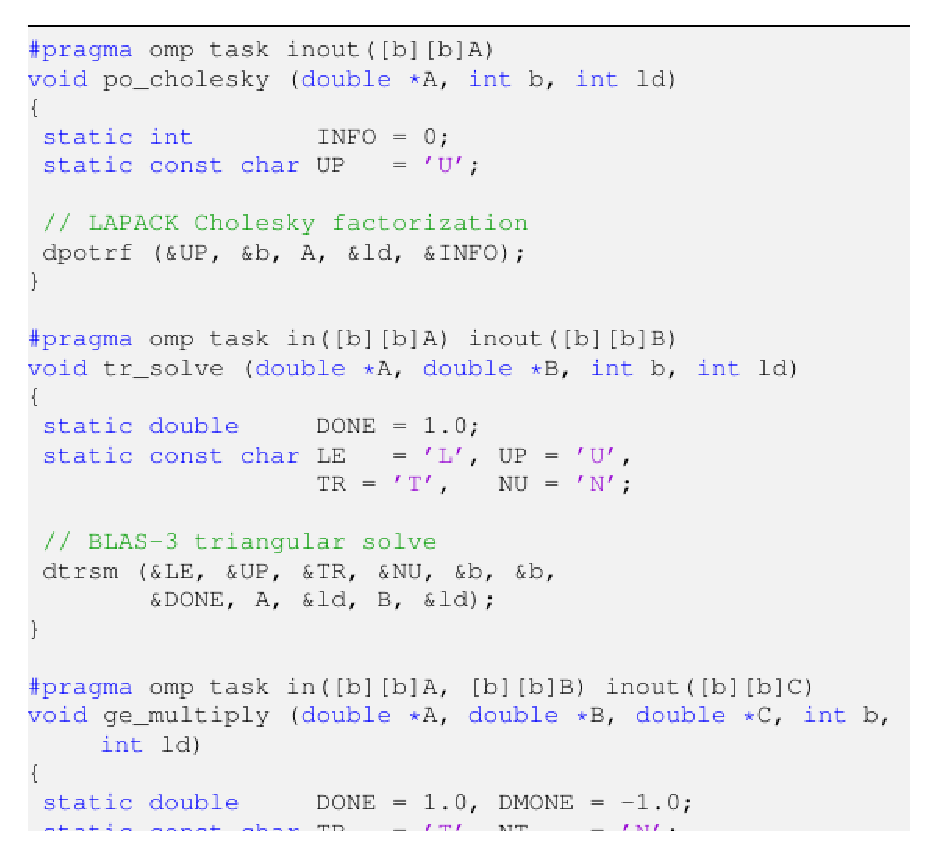
\includegraphics[width=\columnwidth]{Figures/cholesky_tasks.eps}
    \end{column}
    \begin{column}{0.1\textwidth}
      $\xrightarrow{\text{DAG}}$
    \end{column}
    \begin{column}{0.20\textwidth}
      \begin{figure}[tbh!]
        \begin{center}
          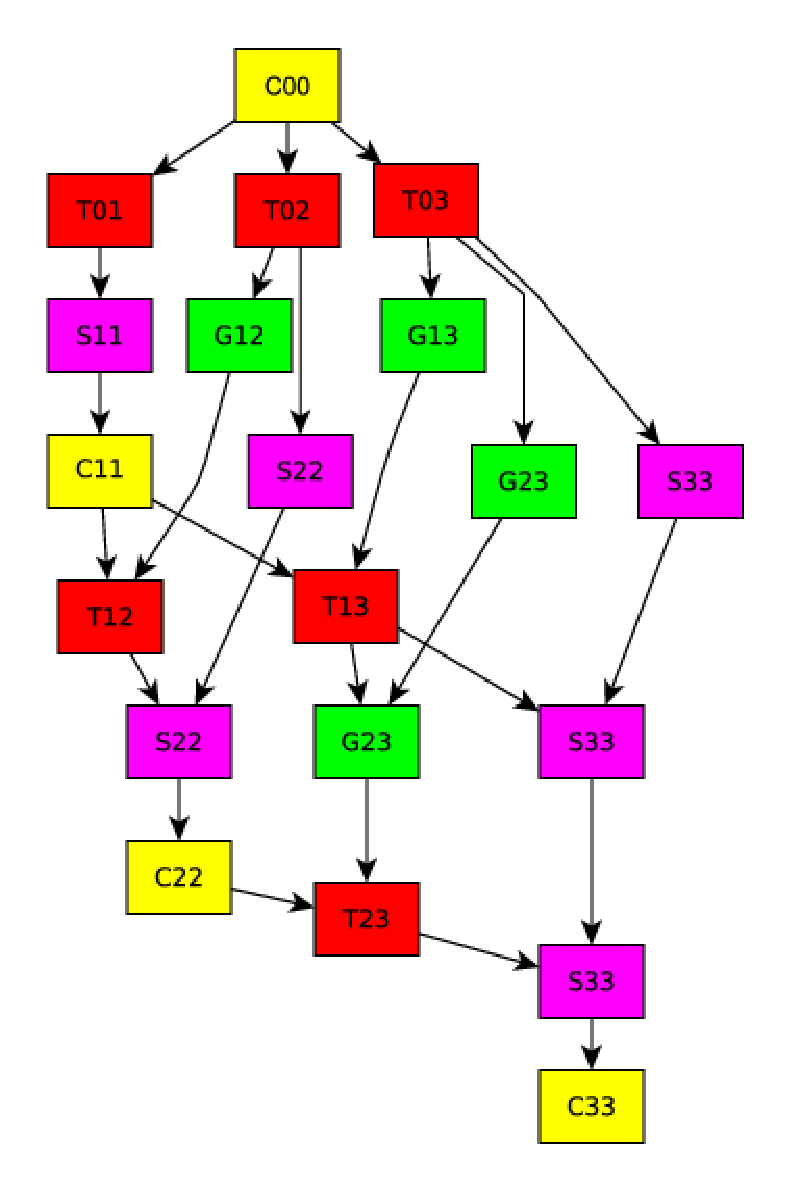
\includegraphics[scale=0.15]{Figures/4x4_TaskExample}
        \end{center}
      \end{figure}
    \end{column}
    \begin{column}{0.1\textwidth}
      $\xrightarrow{\text{Planificación}}$
    \end{column}
    \begin{column}{0.25\textwidth}
      \centering
      \fboxsep=2mm \fboxrule=.5mm
      \fcolorbox{black}{blue!50!white}{\scriptsize BIG0}
      \fboxsep=1.5mm \fboxrule=.5mm
      \fcolorbox{black}{blue!10!white}{\tiny LITTLE0}

      \fboxsep=2mm \fboxrule=.5mm
      \fcolorbox{black}{blue!50!white}{\scriptsize BIG1}
      \fboxsep=1.5mm \fboxrule=.5mm
      \fcolorbox{black}{blue!10!white}{\tiny LITTLE1}

      \fboxsep=2mm \fboxrule=.5mm
      \fcolorbox{black}{blue!50!white}{\scriptsize BIG2}
      \fboxsep=1.5mm \fboxrule=.5mm
      \fcolorbox{black}{blue!10!white}{\tiny LITTLE2}

      \fboxsep=2mm \fboxrule=.5mm
      \fcolorbox{black}{blue!50!white}{\scriptsize BIG3}
      \fboxsep=1.5mm \fboxrule=.5mm
      \fcolorbox{black}{blue!10!white}{\tiny LITTLE3}

    \end{column}
    \begin{column}{0.1\textwidth}
      \rotatebox{90}{Runtime}
    \end{column}
  \end{columns}
\end{frame}

% \begin{frame}
%   \frametitle{Extracción del paralelismo en AMPs: Planificador de tareas}
%   \begin{columns}[c]%[onlytextwidth]
%     \begin{column}{0.25\textwidth}
%       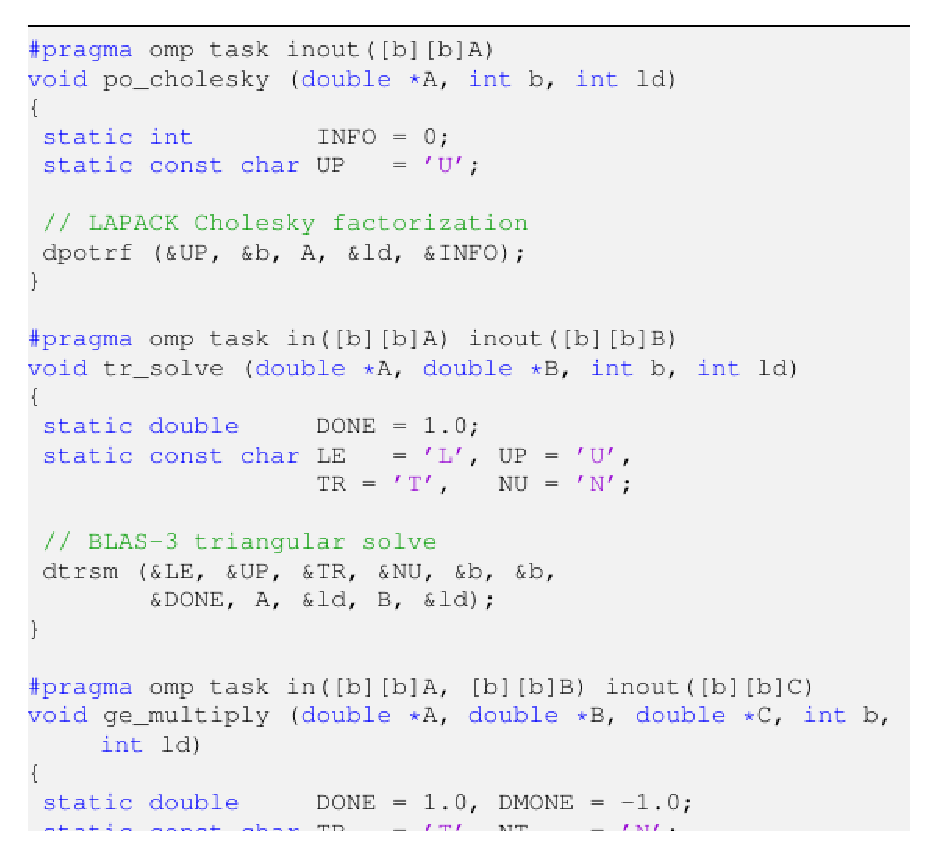
\includegraphics[width=\columnwidth]{Figures/cholesky_tasks.eps}
%     \end{column}
%     \begin{column}{0.1\textwidth}
%       $\xrightarrow{\text{Creación DAG}}$
%     \end{column}
%     \begin{column}{0.25\textwidth}
%       \begin{figure}[tbh!]
%         \begin{center}
%           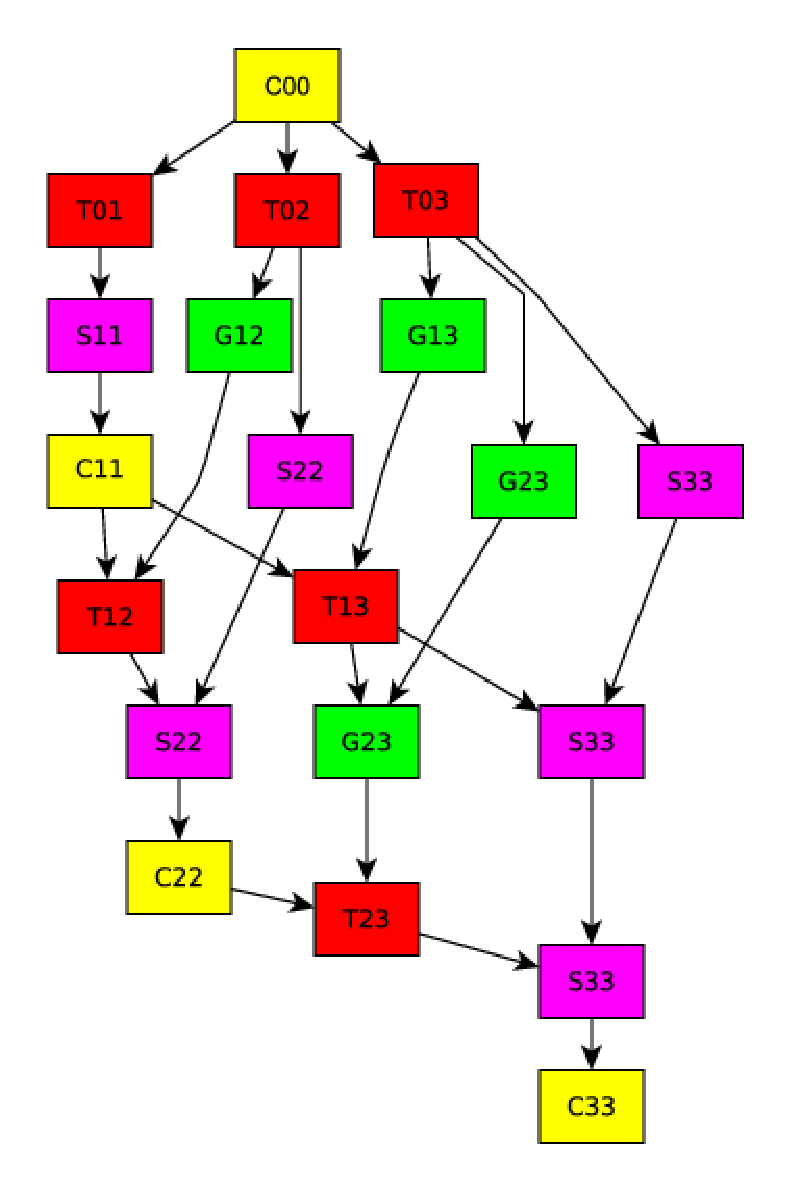
\includegraphics[scale=0.15]{Figures/4x4_TaskExample}
%         \end{center}
%       \end{figure}
%     \end{column}
%     \begin{column}{0.1\textwidth}
%       $\xrightarrow{\text{Planificación tarea}}$
%     \end{column}
%     \begin{column}{0.25\textwidth}
%       \centering
%       \fboxsep=2mm \fboxrule=.5mm
%       \fcolorbox{black}{blue!50!white}{\tiny CPU0}

%       \fcolorbox{black}{blue!50!white}{\tiny CPU1}

%       \fcolorbox{black}{blue!50!white}{\tiny CPU2}

%       \fcolorbox{black}{blue!50!white}{\tiny CPU3}
%     \end{column}
%   \end{columns}

%   \vfill

%   \begin{itemize}
%   \item {\bf Ventajas:} Facilidad de programar, en general.
%   \item {\bf Inconvenientes:} Políticas de planificación complejas.
%   \end{itemize}  
% \end{frame}


\begin{frame}
  \frametitle{Extracción del paralelismo en AMPs: Biblioteca}
  \begin{figure}[th!]
    \begin{center}
      \includegraphics[width=0.5\columnwidth]{Figures/A15vsA7.pdf}
    \end{center}
    \caption{\label{fig:A15vsA7} Distribución de la carga de trabajo para
      una multiplicación de matrices $C \mathrel{+}= A \cdot B$
      entre los clusters A15 y A7, sobre la librería BLIS.}
  \end{figure}

  \begin{itemize}
  \item {\bf Ventajas:} Específica para una aplicación y arquitectura concreta.
  \item {\bf Inconvenientes:} Implementación específica para una arquitectura.
  \end{itemize}    
\end{frame}


%===========================================================================
\section{Optimización del rendimiento}
\begin{frame}
  \frametitle{Necesidad de explotar la asimetría}
  \begin{figure}\centering
    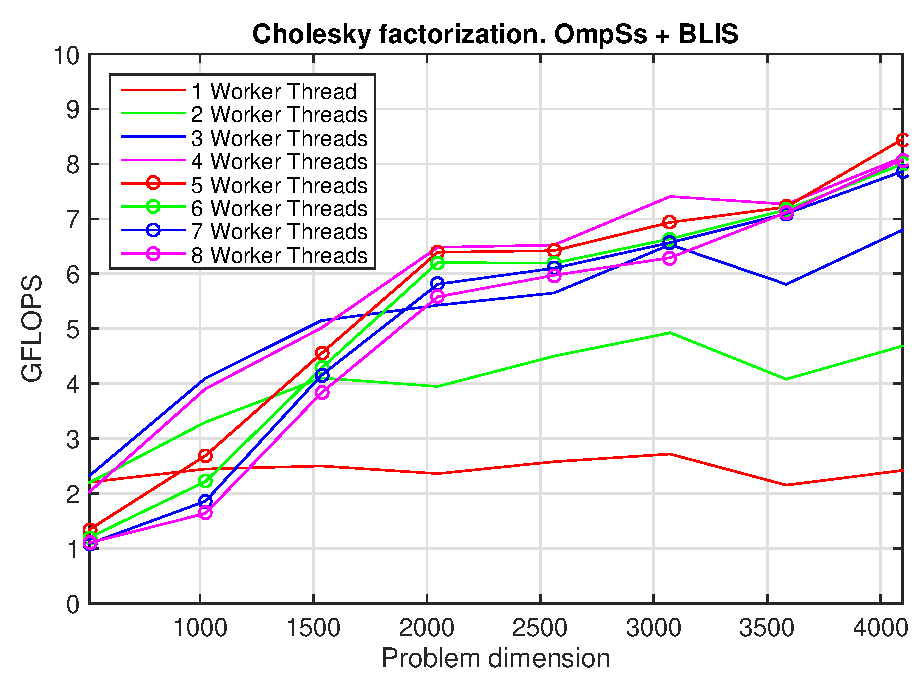
\includegraphics[width=0.65\textwidth]{Plots/Orig_runtime/plot_1to8_th.eps}
  \end{figure}

  \begin{itemize}
  \item Necesario explorar o adaptar nuevas técnicas para obtener un alto
    rendimiento.
  \end{itemize}
\end{frame}

\begin{frame}
  \frametitle{Planificadores de tareas sobre AMPs}
  {\bf ¿Cómo explotar la asimetría mediante un planificador de tareas?}

  \begin{block}{Opción 1: {\bf Planificador de tareas específico}}
    \begin{itemize}
      \footnotesize
    \item Ya implementado por el BSC: {\bf Botlev}.
    \item Un {\em worker thread} por cada núcleo físico.
    \item Las tareas invocan a bibliotecas {\bf secuenciales}.
    \item El planificador acelera la ejecución del camino crítico:
      mapeado de tareas críticas sobre núcleos rápidos.
%    \item Robo de tareas entre ambos clusters.
    \end{itemize}
  \end{block}

  \begin{alertblock}{Opción 2: {\bf Planificador convencional} + {\bf biblioteca asimétrica}}
    \begin{itemize}
      \footnotesize
    \item Para el planificador, la arquitectura es simétrica.
    \item Cada ``núcleo virtual'' (VC) está compuesto por un pareja de
      núcleos big+LITTLE.
    \item Un {\em worker thread} por cada {\bf núcleo virtual}.
    \item Las tareas invocan rutinas sobre una biblioteca {\bf
        asimétrica} (ej. BLIS).
    \end{itemize}
  \end{alertblock}
\end{frame}

\begin{frame}
  \frametitle{Planificadores de tareas sobre AMPs}
  {\footnotesize Opción 1:}

  \begin{columns}[c]%[onlytextwidth]
    \begin{column}{0.3\textwidth}
      \begin{figure}[tbh!]
        \begin{center}
          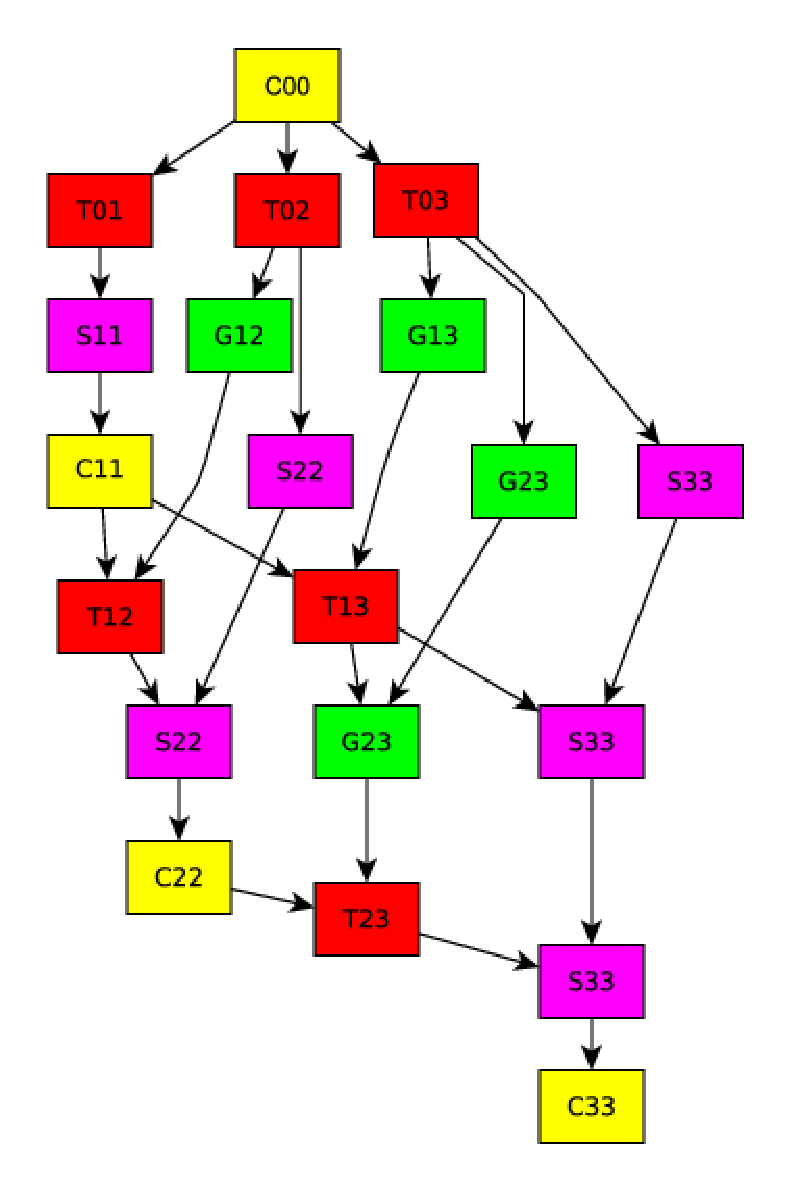
\includegraphics[scale=0.12]{Figures/4x4_TaskExample}
        \end{center}
      \end{figure}
    \end{column}
    \begin{column}{0.2\textwidth}
      $\xrightarrow[\text{8 workers + Biblioteca Sec.}]{\text{Planificador Ad-hoc}}$
    \end{column}
    \begin{column}{0.4\textwidth}
      \centering
      \fboxsep=1mm \fboxrule=.5mm
      \fcolorbox{black}{blue!50!white}{\footnotesize BIG0}

      \fcolorbox{black}{blue!50!white}{\footnotesize BIG1}

      \fcolorbox{black}{blue!50!white}{\footnotesize BIG2}

      \fcolorbox{black}{blue!50!white}{\footnotesize BIG3}

      \fboxsep=.5mm \fboxrule=.5mm
      \fcolorbox{black}{blue!10!white}{\tiny LITTLE0}

      \fcolorbox{black}{blue!10!white}{\tiny LITTLE1}

      \fcolorbox{black}{blue!10!white}{\tiny LITTLE2}

      \fcolorbox{black}{blue!10!white}{\tiny LITTLE3}
    \end{column}
  \end{columns}

  {\footnotesize Opción 2:}

  \begin{columns}[c]%[onlytextwidth]
    \begin{column}{0.3\textwidth}
      \begin{figure}[tbh!]
        \begin{center}
          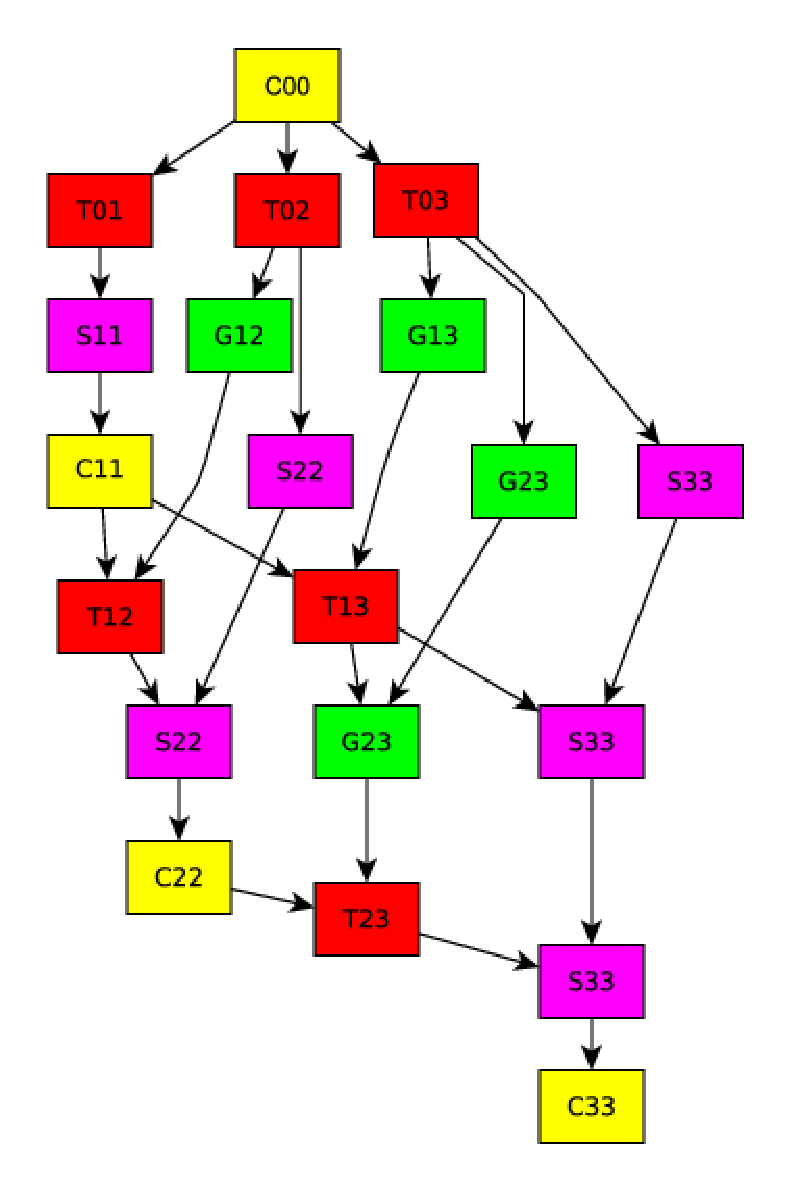
\includegraphics[scale=0.12]{Figures/4x4_TaskExample}
        \end{center}
      \end{figure}
    \end{column}
    \begin{column}{0.2\textwidth}
      $\xrightarrow[\text{4 workers + Biblioteca Asim.}]{\text{Planificador
          convencional}}$
    \end{column}
    \begin{column}{0.4\textwidth}
      \centering
      \fboxsep=.1mm \fboxrule=.5mm
      \fcolorbox{black}{blue!0!white}{\tiny VC0 \linebreak
        \fboxsep=1mm \fboxrule=.2mm
        \fcolorbox{black}{blue!50!white}{\footnotesize BIG0}
        \fboxsep=.5mm \fboxrule=.2mm
        \fcolorbox{black}{blue!10!white}{\tiny LITTLE0}
      }

      \fboxsep=.1mm \fboxrule=.5mm
      \fcolorbox{black}{blue!0!white}{\tiny VC1 \linebreak
        \fboxsep=1mm \fboxrule=.2mm
        \fcolorbox{black}{blue!50!white}{\footnotesize BIG1}
        \fboxsep=.5mm \fboxrule=.2mm
        \fcolorbox{black}{blue!10!white}{\tiny LITTLE1}
      }

      \fboxsep=.1mm \fboxrule=.5mm
      \fcolorbox{black}{blue!0!white}{\tiny VC2 \linebreak
        \fboxsep=1mm \fboxrule=.2mm
        \fcolorbox{black}{blue!50!white}{\footnotesize BIG2}
        \fboxsep=.5mm \fboxrule=.2mm
        \fcolorbox{black}{blue!10!white}{\tiny LITTLE2}
      }

      \fboxsep=.1mm \fboxrule=.5mm
      \fcolorbox{black}{blue!0!white}{\tiny VC3 \linebreak
        \fboxsep=1mm \fboxrule=.2mm
        \fcolorbox{black}{blue!50!white}{\footnotesize BIG3}
        \fboxsep=.5mm \fboxrule=.2mm
        \fcolorbox{black}{blue!10!white}{\tiny LITTLE3}
      }

    \end{column}
  \end{columns}
\end{frame}


\begin{frame}
  \frametitle{Resultados (I)}
  \begin{figure}
    \centering
    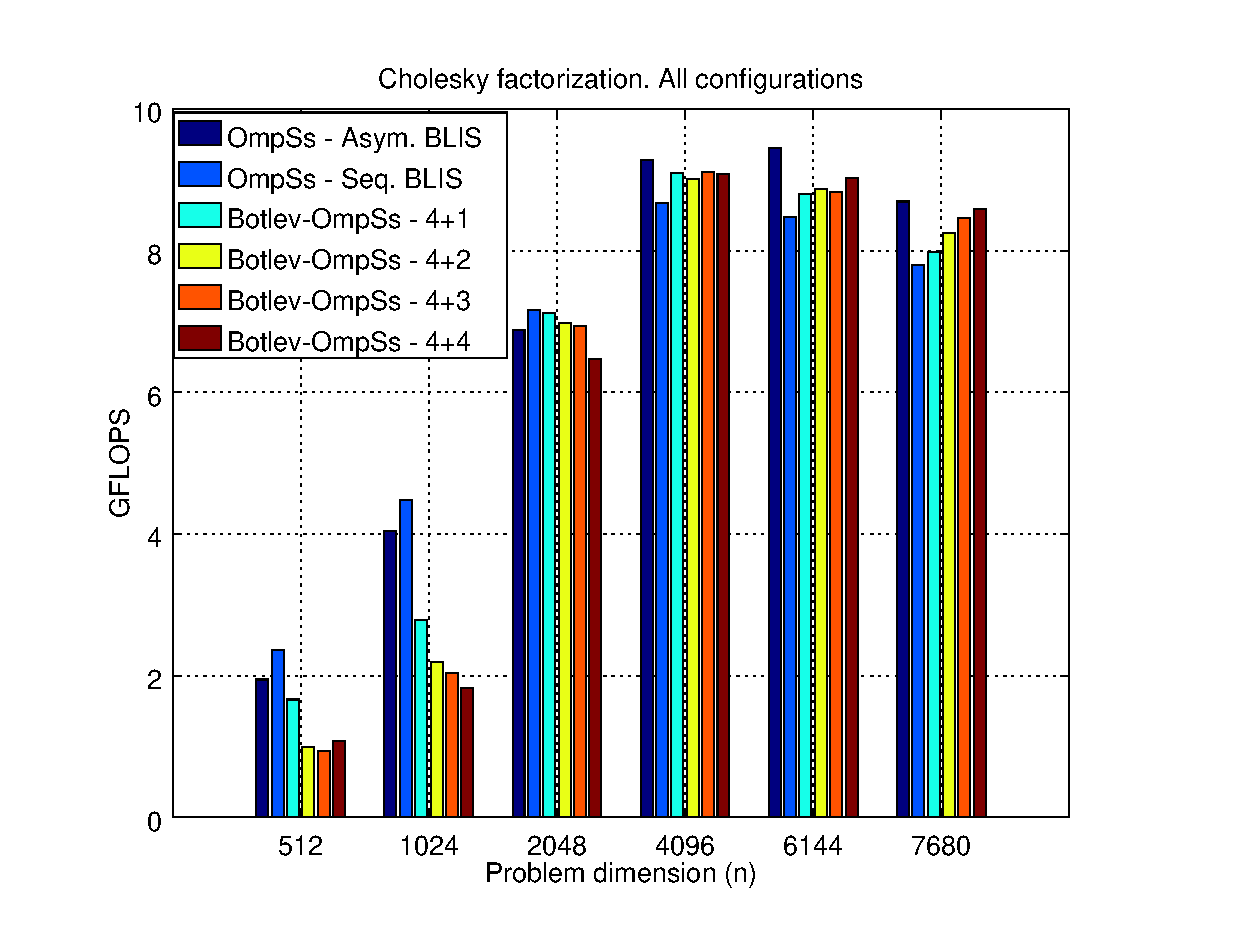
\includegraphics[width=0.65\textwidth]{Plots/Comparative/comparative}
    \caption{Rendimiento para la factorización de Cholesky utilizando el
      planificador convencional de OmpSs enlazado con la versión secuencial
      de BLIS, la implementación asimétrica de BLIS, y la implementación
      consciente de la asimetría Botlev de Ompss.}
    \label{fig:comparative}
  \end{figure}
\end{frame}


\begin{frame}
  \frametitle{Resultados (II)}
  \begin{figure}%[t]
    \centering
    \tiny
    \subfigure[\tiny OmpSs - Sequential BLIS (8 worker threads)]{
      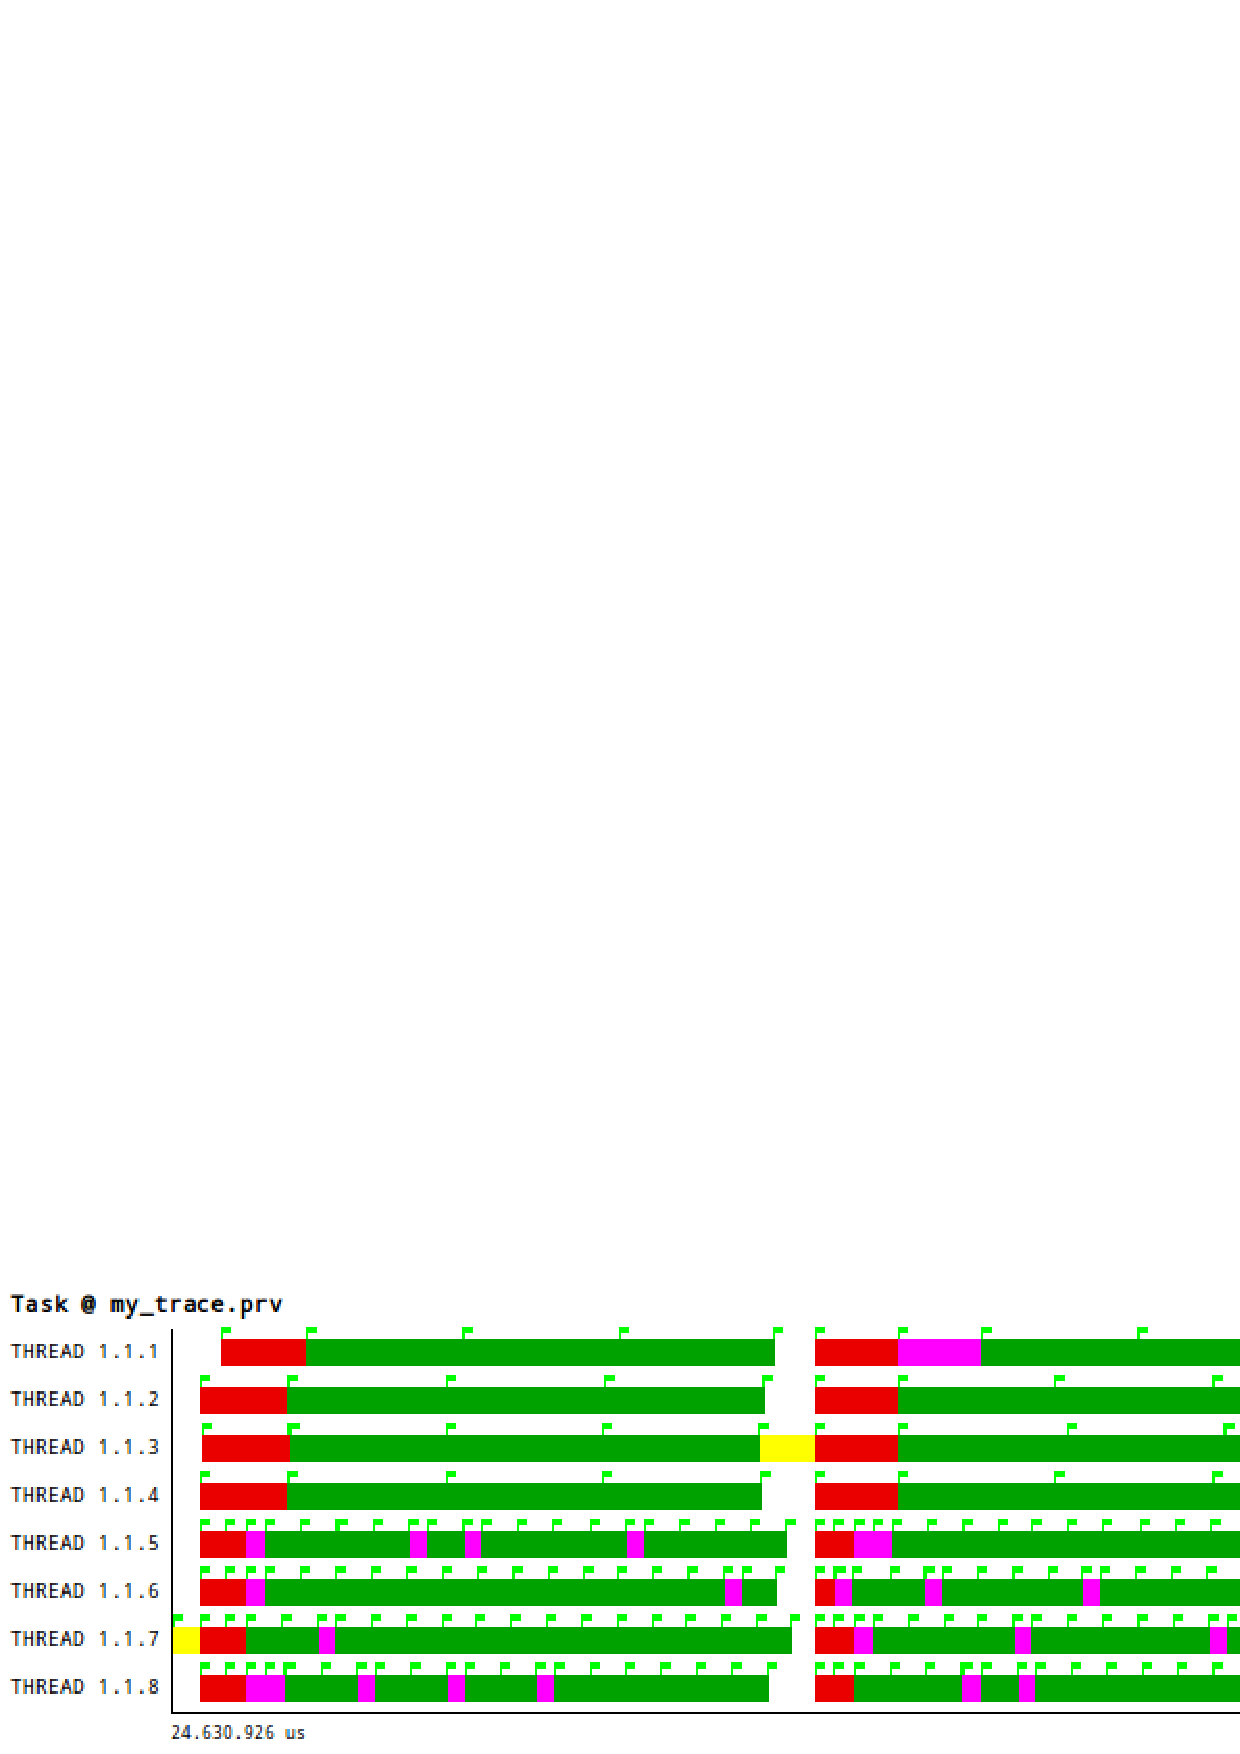
\includegraphics[width=0.95\textwidth]{Plots/Traces/sym_8cores_tasks.png}
    }
    \subfigure[\tiny OmpSs - Sequential BLIS (4 worker threads)]{
      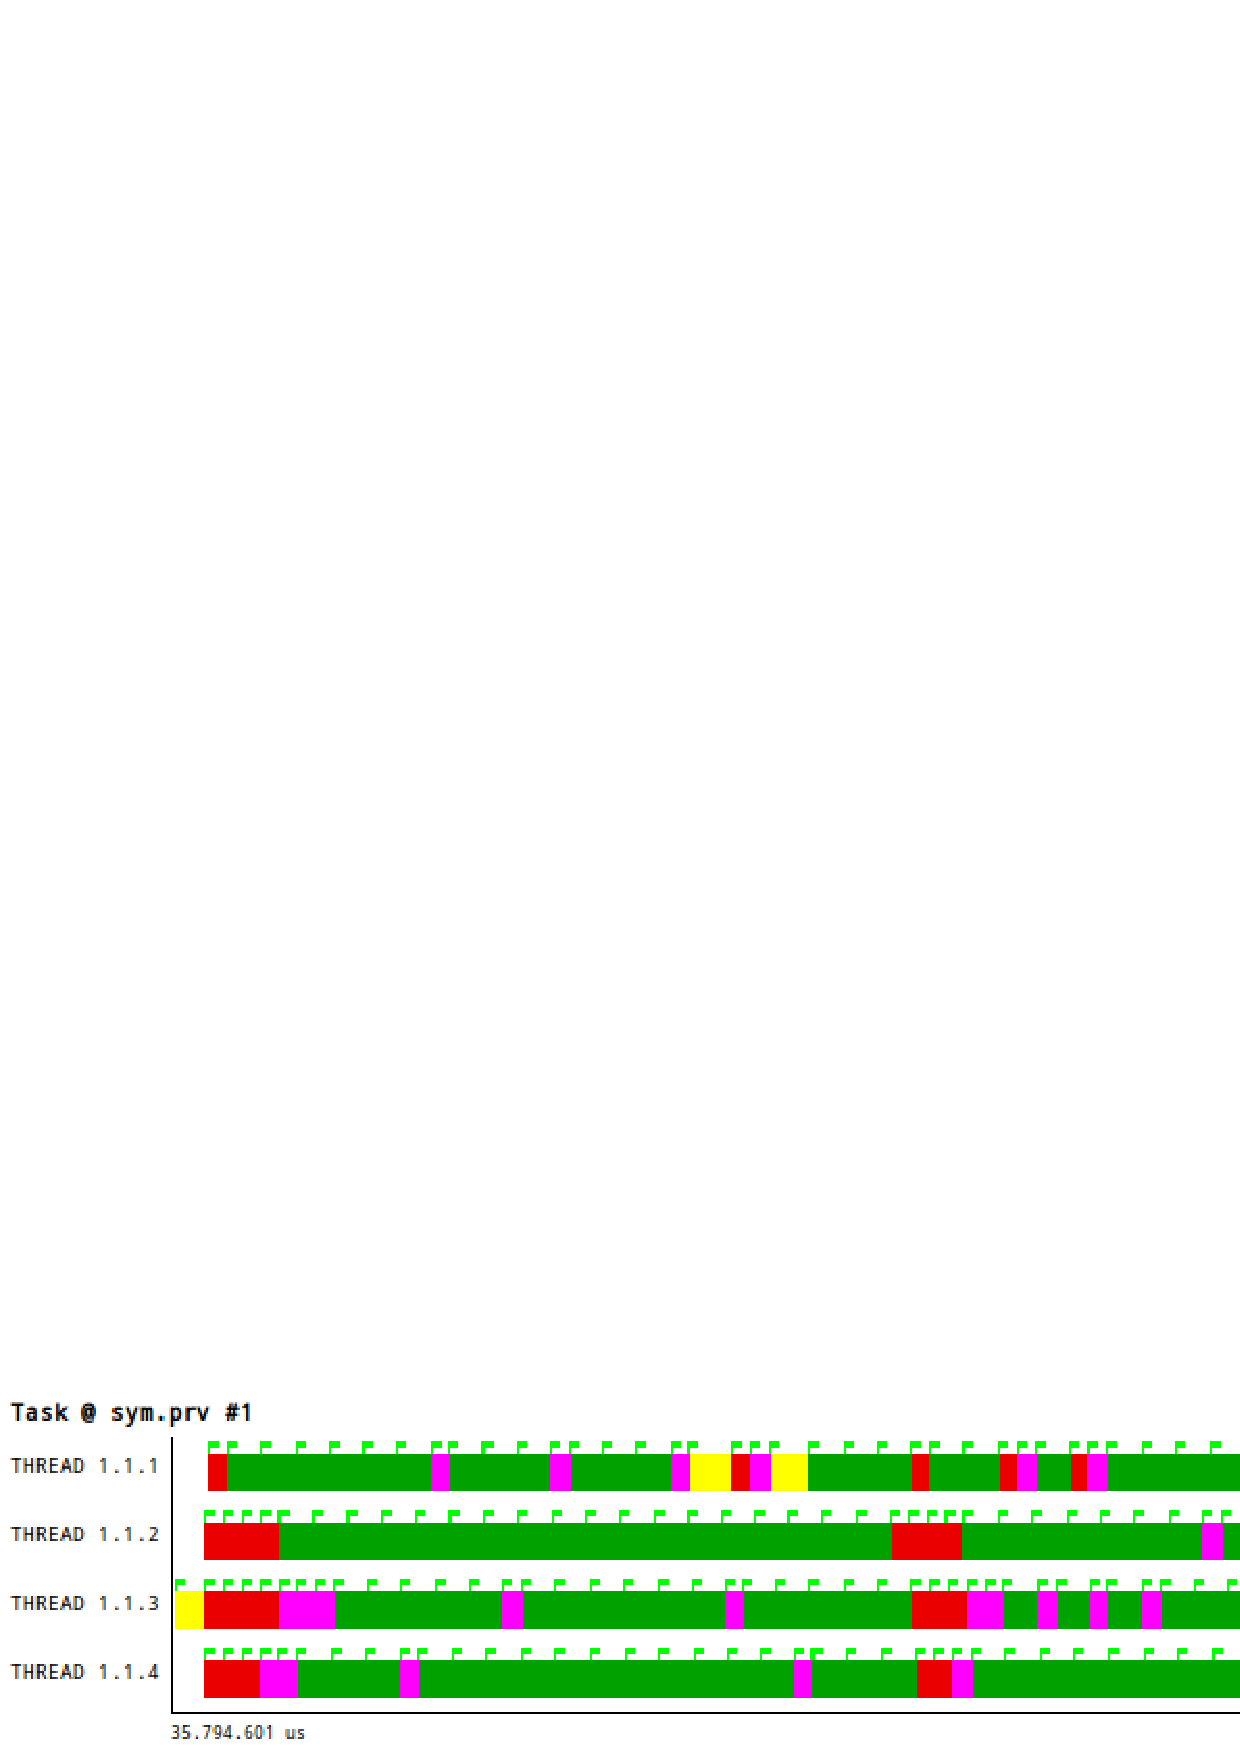
\includegraphics[width=0.95\textwidth]{Plots/Traces/sym_tasks.png}
    }
    \subfigure[\tiny \bf OmpSs - Asymmetric BLIS (4 worker threads)]{
      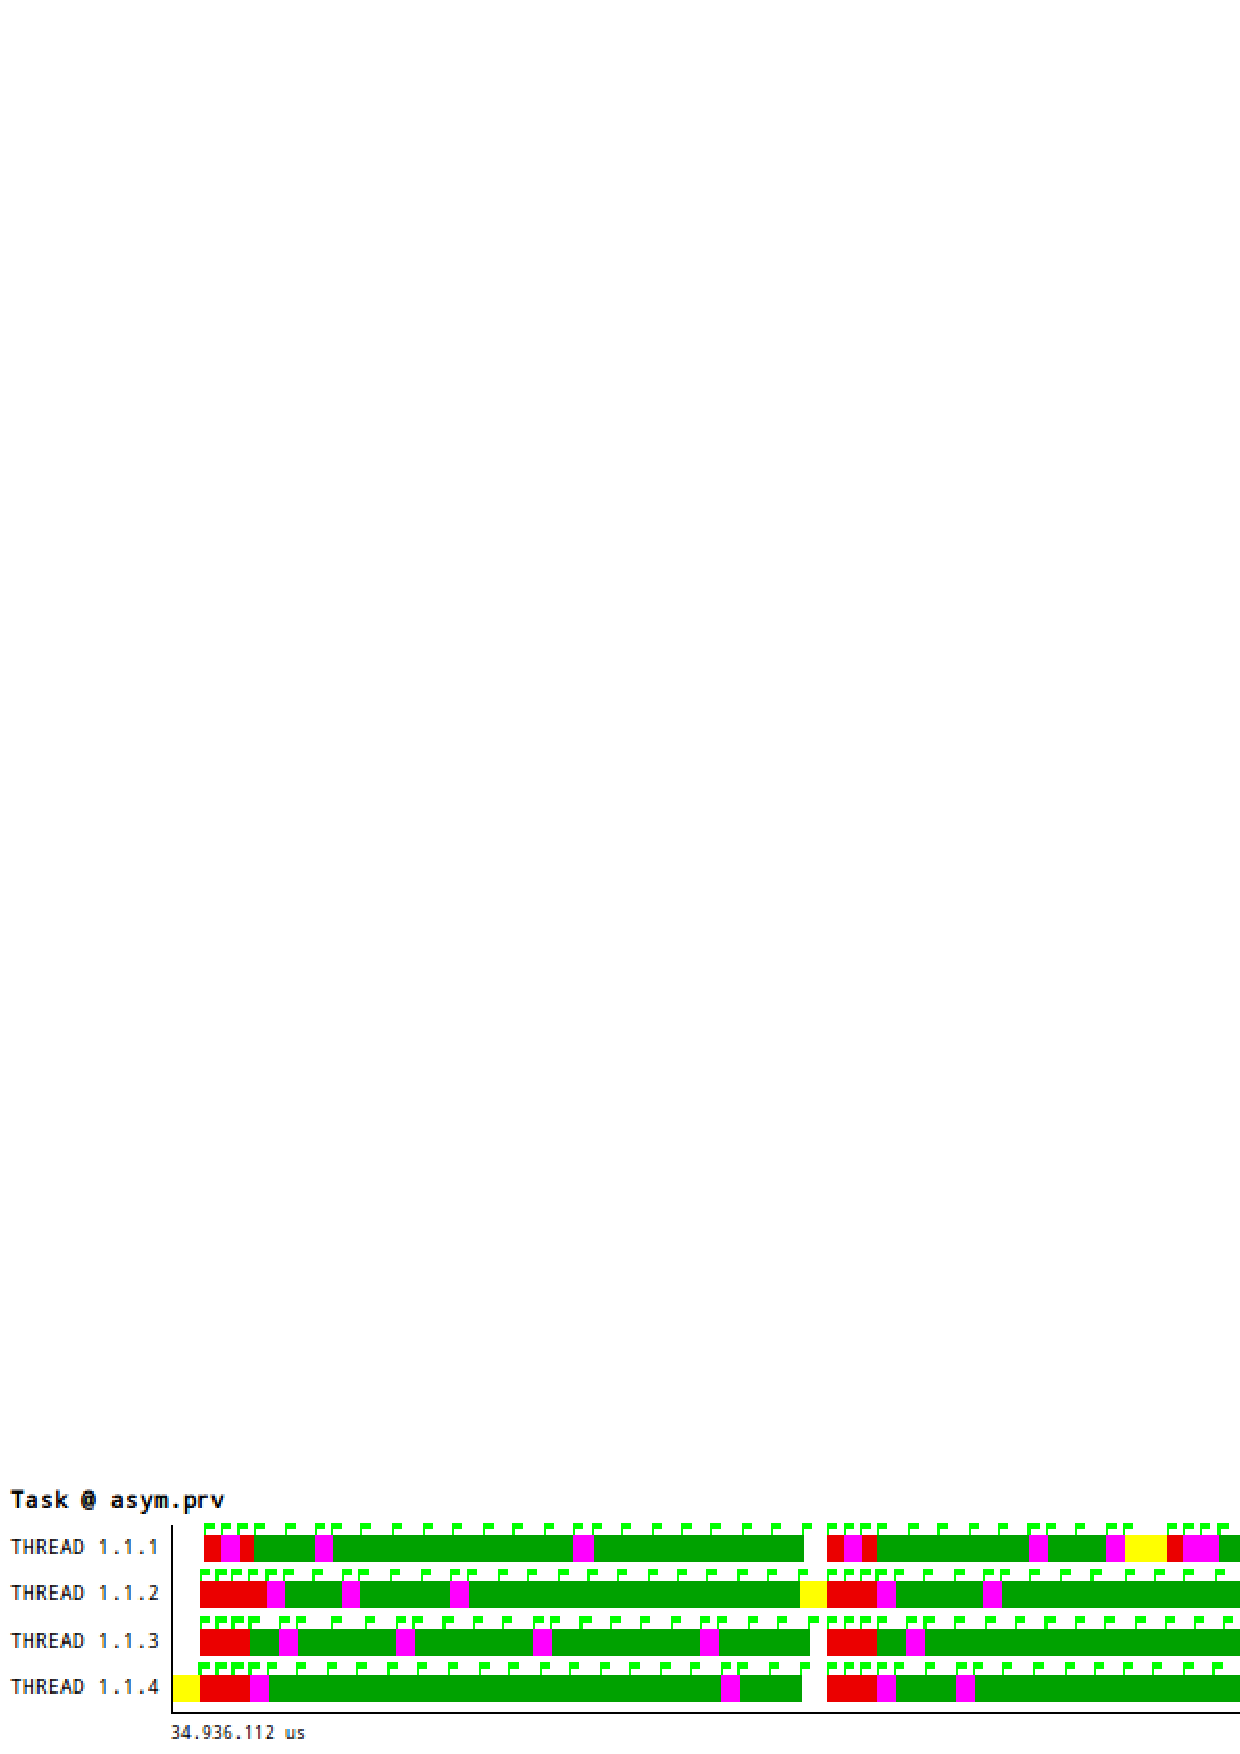
\includegraphics[width=0.95\textwidth]{Plots/Traces/asym_tasks.png}
    }
    \subfigure[\tiny Botlev-OmpSs - Sequential BLIS (8 worker threads, 4+4)]{
      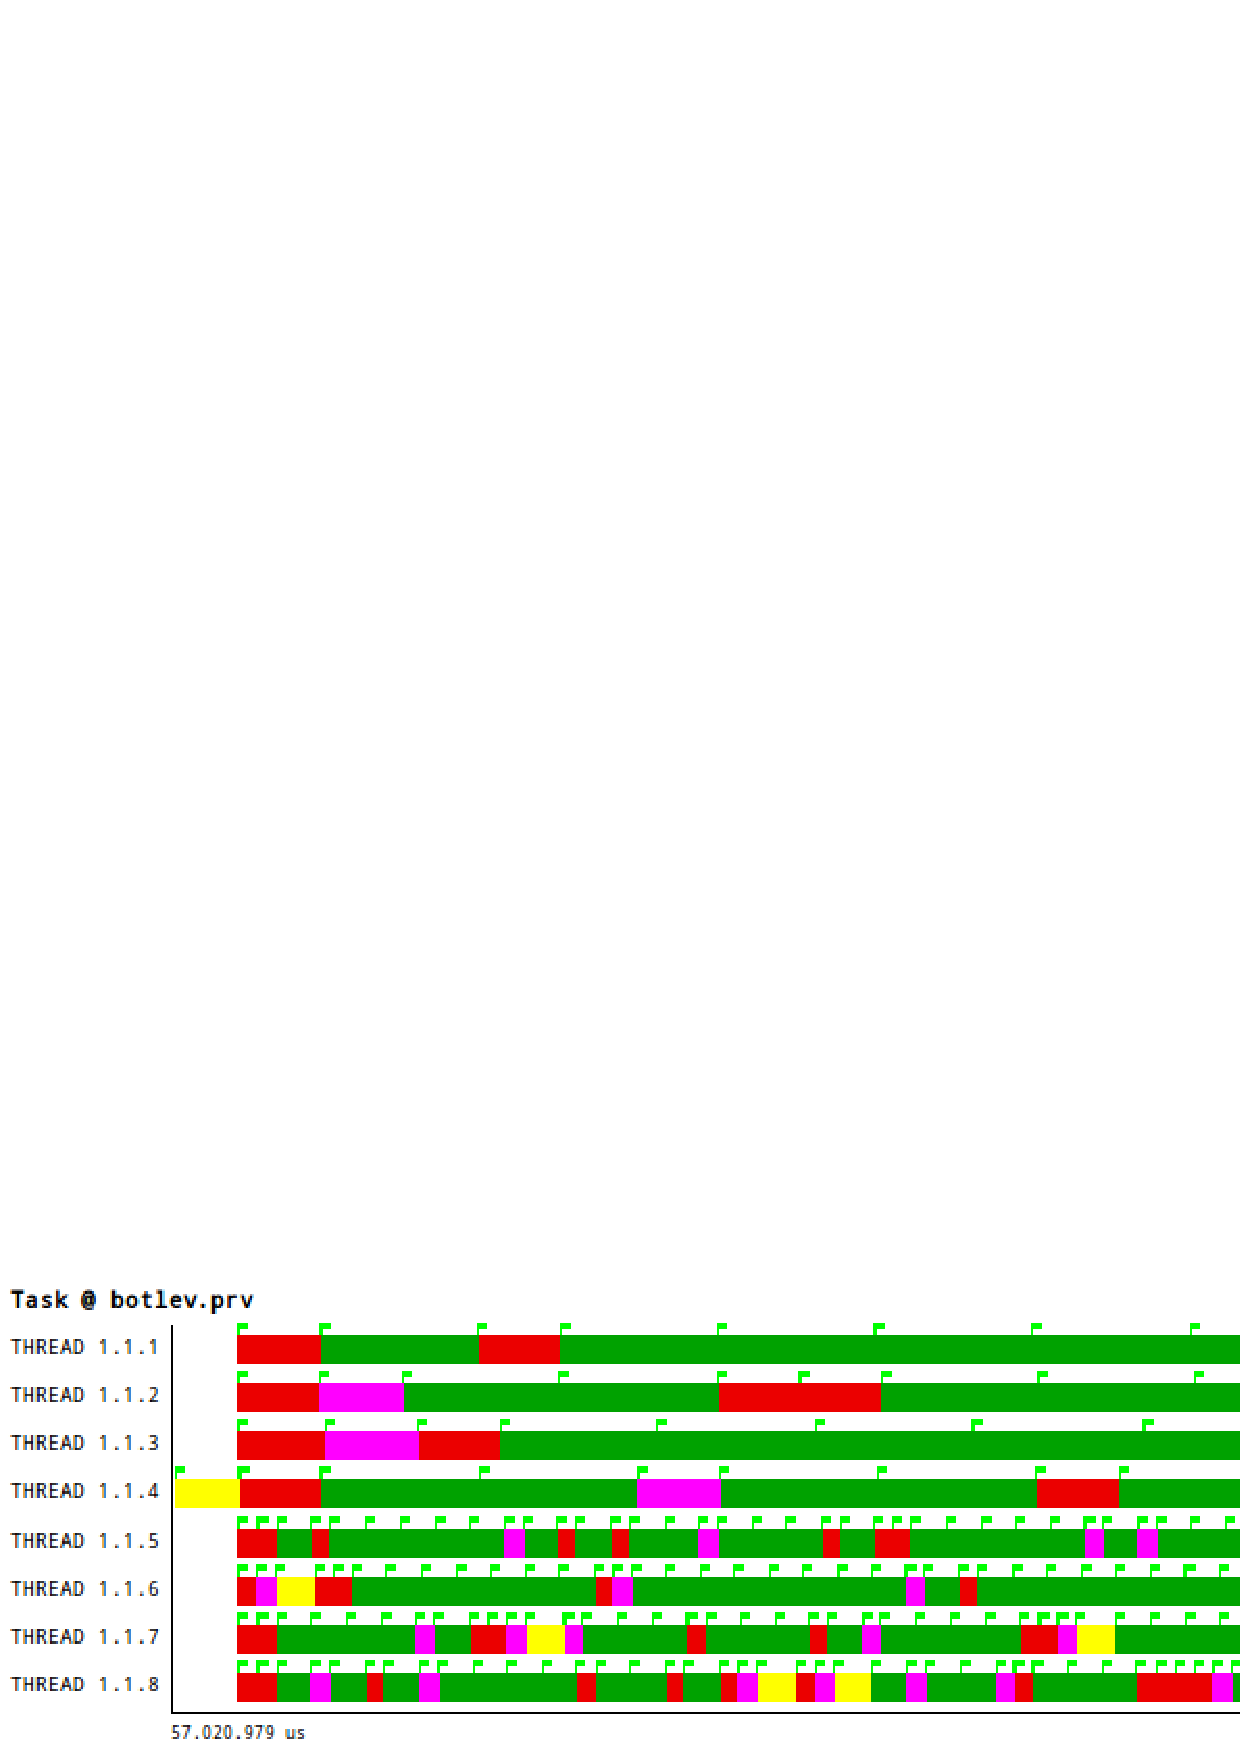
\includegraphics[width=0.95\textwidth]{Plots/Traces/botlev_tasks.png}
    }
    
    \label{fig:traces_tasks}
  \end{figure}
  
  \begin{center}
    Factorización de Cholesky por bloques, $n=6144$. Traza de planificación
    de tareas.
  \end{center}
\end{frame}
%===========================================================================
\section{Optimización de la eficiencia energética}

\begin{frame}
  \frametitle{Medidas de consumo}
  \begin{columns}
    \begin{column}{0.4\textwidth}
      \begin{center}
        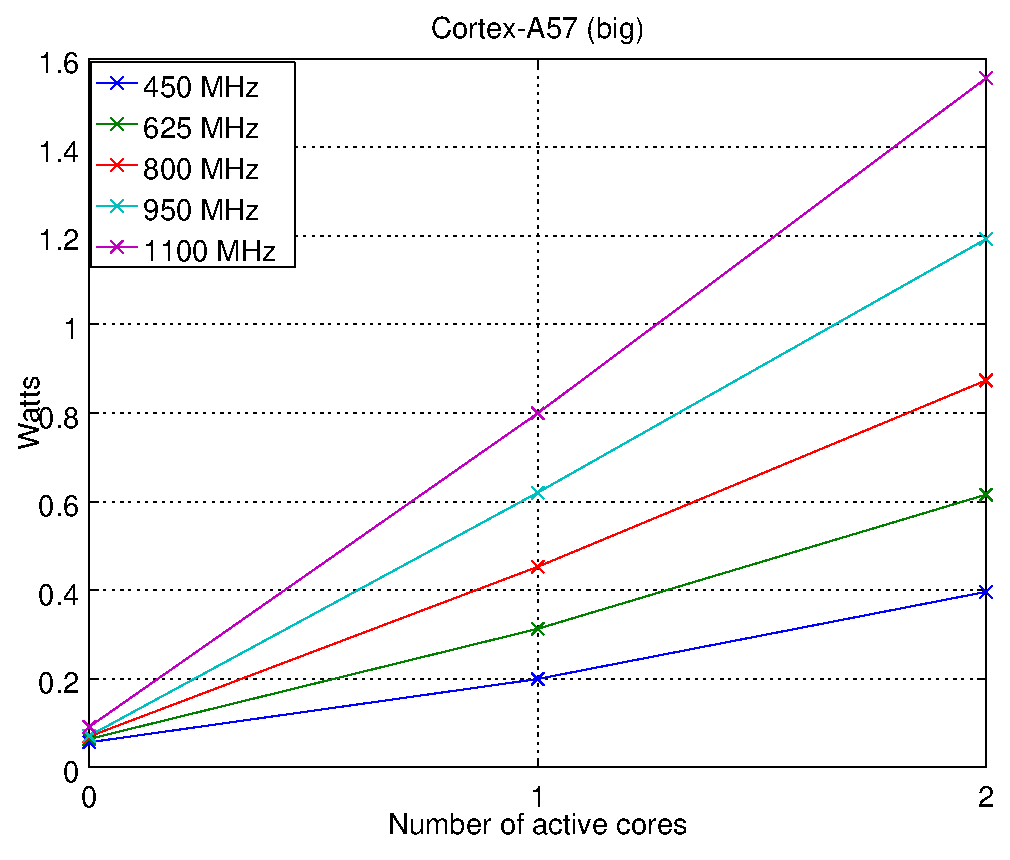
\includegraphics[width=0.9\textwidth]{Plots/modelo_consumo/juno_big.eps}\\\vspace{0.2cm}
        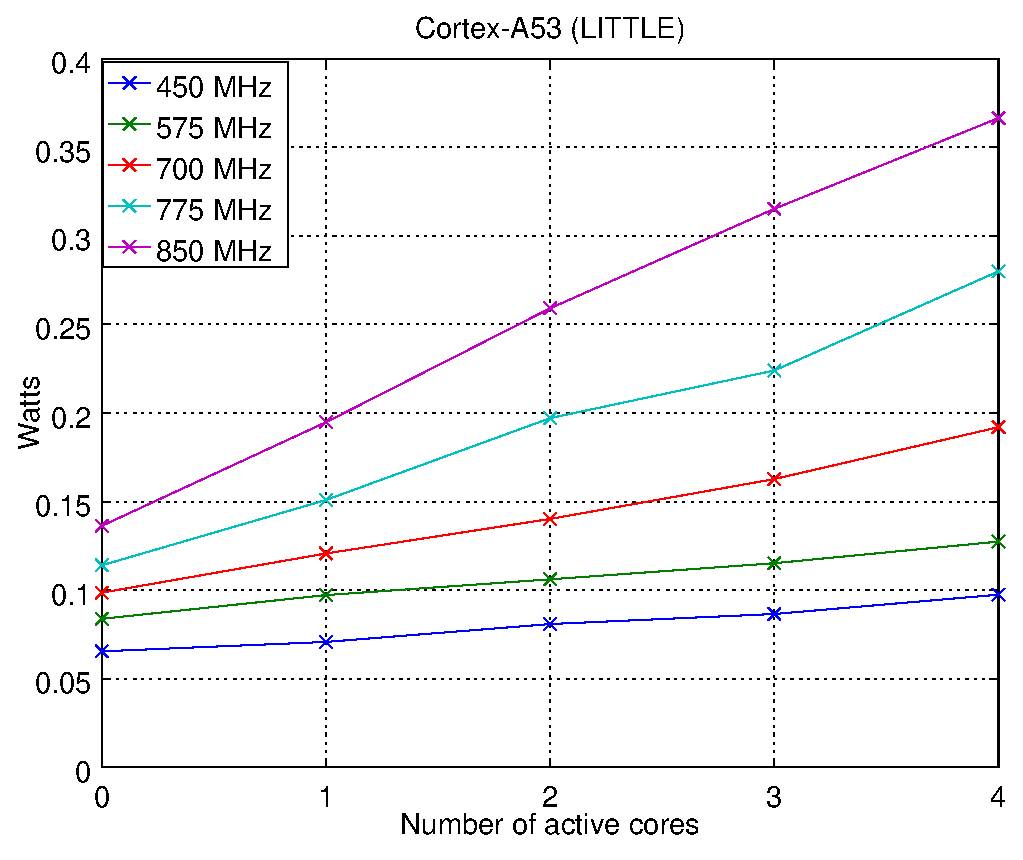
\includegraphics[width=0.9\textwidth]{Plots/modelo_consumo/juno_little.eps}\\
      {\centering \footnotesize {\sc Juno} (4 LITTLE + 2 big)}
      \end{center}
      
    \end{column}
    \begin{column}{0.4\textwidth}
      \begin{center}
        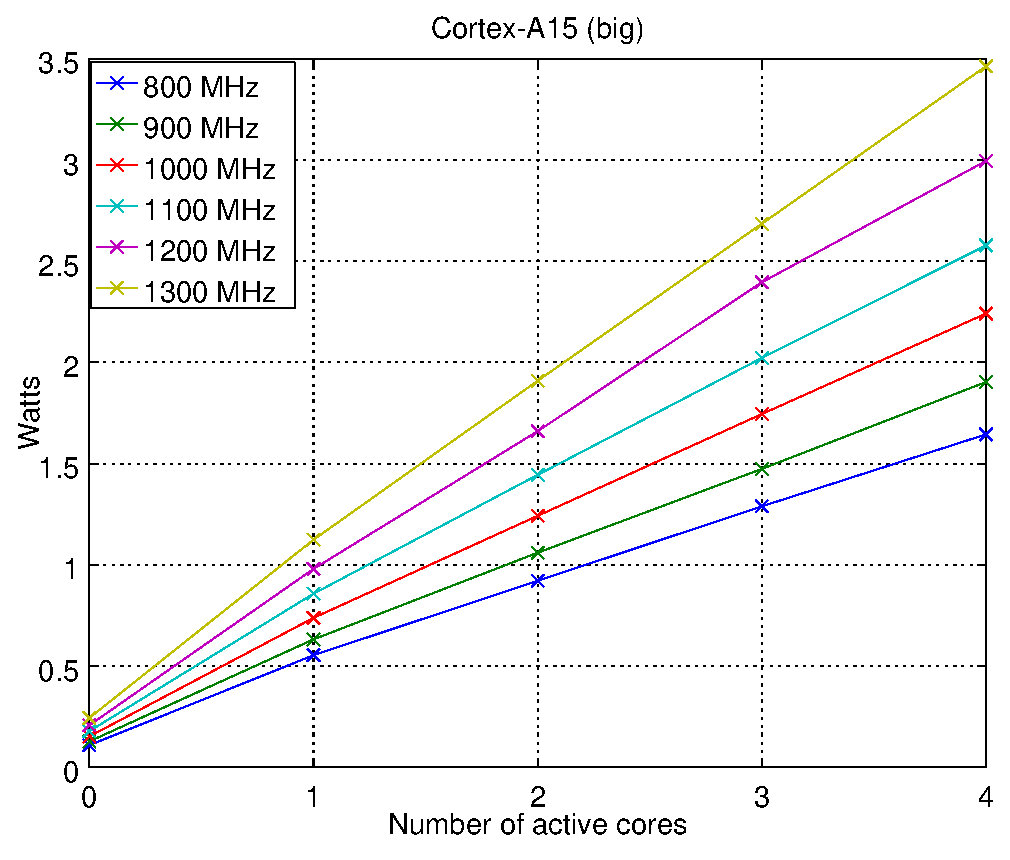
\includegraphics[width=0.9\textwidth]{Plots/modelo_consumo/odroid_big.eps}\\
        \vspace{0.2cm}
        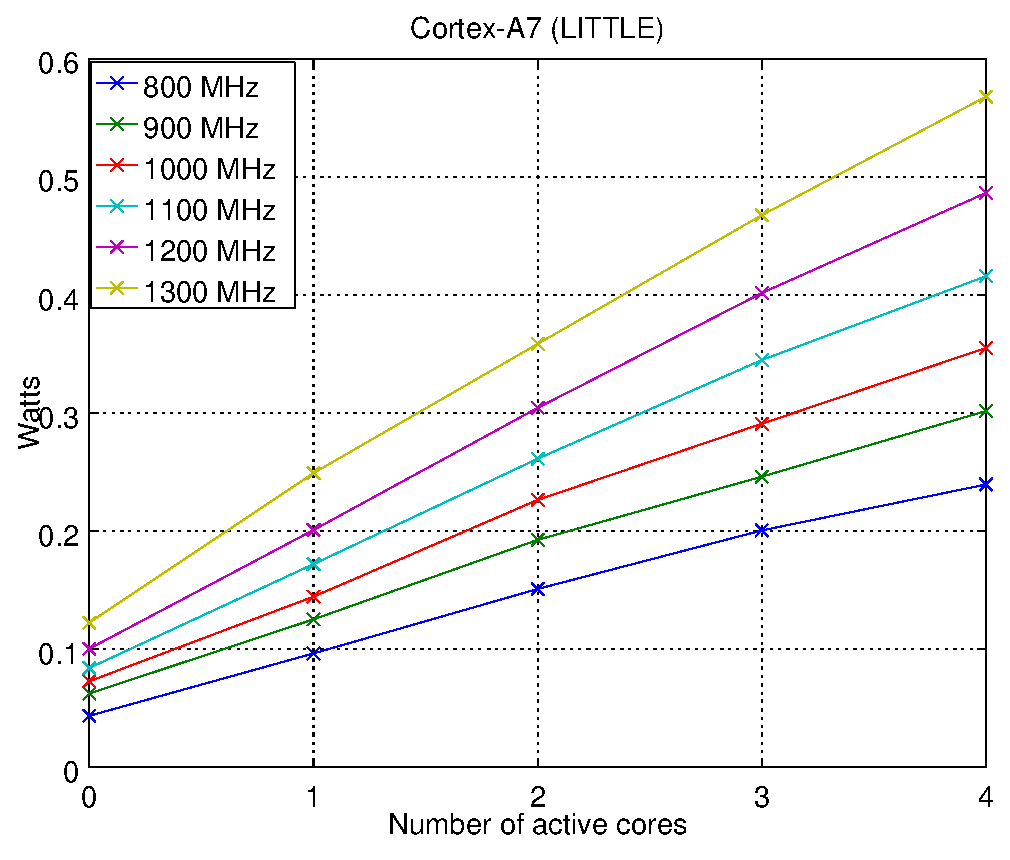
\includegraphics[width=0.9\textwidth]{Plots/modelo_consumo/odroid_little.eps}\\
        {\centering \footnotesize {\sc Odroid} (4 LITTLE + 4 big)}
      \end{center}
      
    \end{column}
  \end{columns}
\end{frame}


\begin{frame}
  \frametitle{Mejora de la eficiencia energética}
  
  \begin{itemize}
  \item Compromiso entre rendimiento y consumo: GFLOPS/Watt.
  \item Disminuir la potencia instantánea $\nRightarrow$ Disminuir el consumo.
  \end{itemize}

  \vfill

  \begin{block}{Opción 1: Técnicas DVFS}
    \begin{itemize}
    \item Modificar el planificador para ser conscientes del nivel de carga
      de trabajo.
    \item Modificar la frecuencia a nivel de cluster.
      \begin{itemize}
      \item ¿Cuándo disminuir/aumentar la frecuencia?
      \item ¿Qué cluster modificar?
      \end{itemize}
    \end{itemize}
  \end{block}

  \begin{block}{Opción 2: Técnicas de planificación}
    \begin{itemize}
    \item Ciertos momentos de la ejecución desactivar un cluster.
    \item Modificar el planificador para realizar la asignación de tareas.
      
      \begin{itemize}
      \item ¿Cuándo desactivar un cluster?
      \item ¿Qué cluster desactivar?
      \end{itemize}
    \end{itemize}
  \end{block}
\end{frame}



\begin{frame}
  \frametitle{Técnicas DVFS}
  {\bf Política P1:} Tareas limitadas por el camino crítico
  \vfill
  \vspace{-0.8cm}
  \begin{figure}
    \centering
    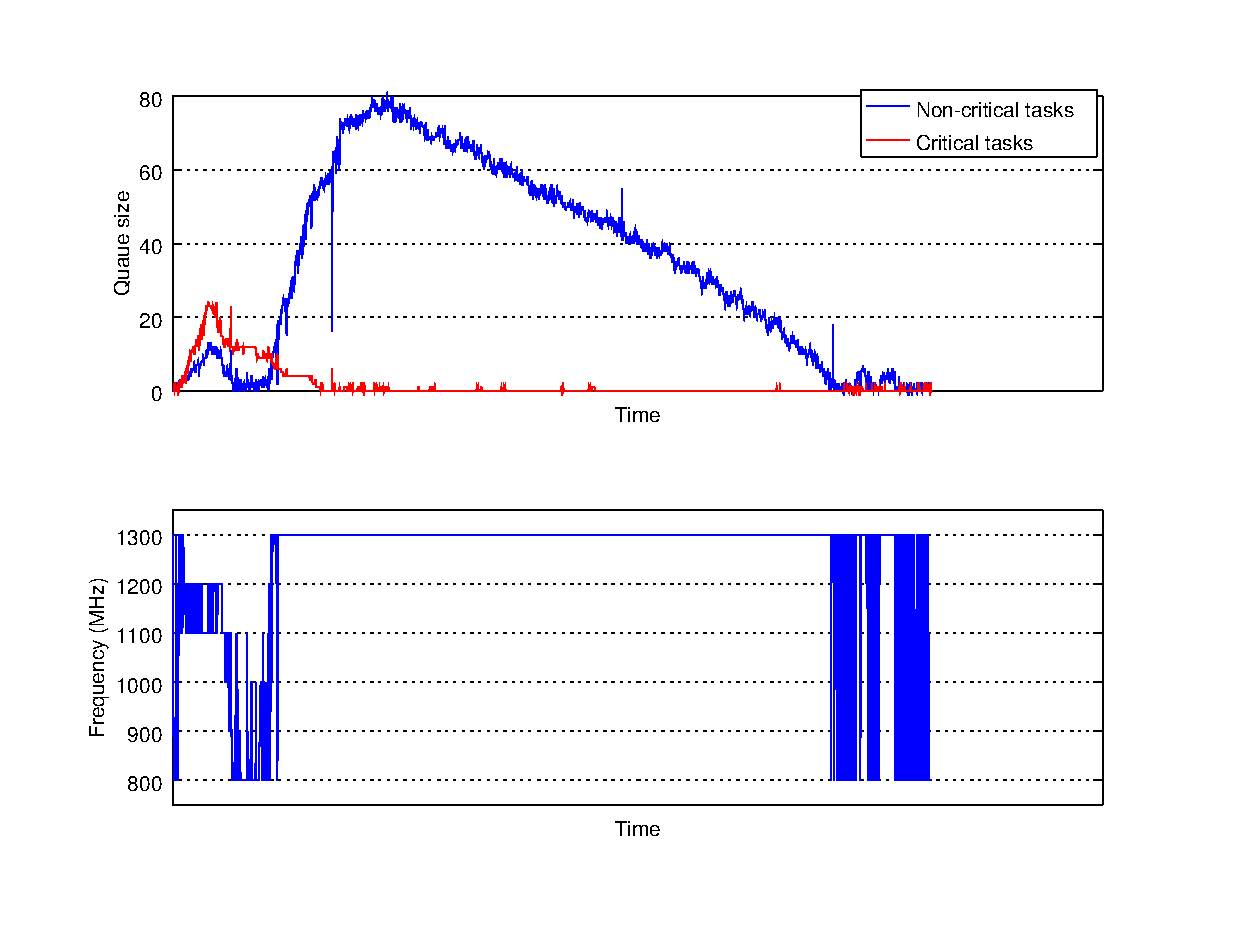
\includegraphics[width=0.9\textwidth]{Plots/politicas/P1_1024-64_juno.eps}
    \vspace{-0.8cm}
    \caption{Factorización de Cholesky con $m=1024$, $b=64$ sobre {\sc Juno}.}
    % \caption{Política P1 sobre una factorización de Cholesky en una matriz
    %   de 1024 elementos dividida en bloques de 64, sobre la plataforma {\sc
    %     Juno}.}
  \end{figure}
  \vspace{-1cm}
\end{frame}

\begin{frame}
  \frametitle{Técnicas DVFS}
  {\bf Políticas P2, P2' y P3:} Escalado del cluster en función de la carga
  \vfill
  \vspace{-0.8cm}
  \begin{figure}
    \centering
    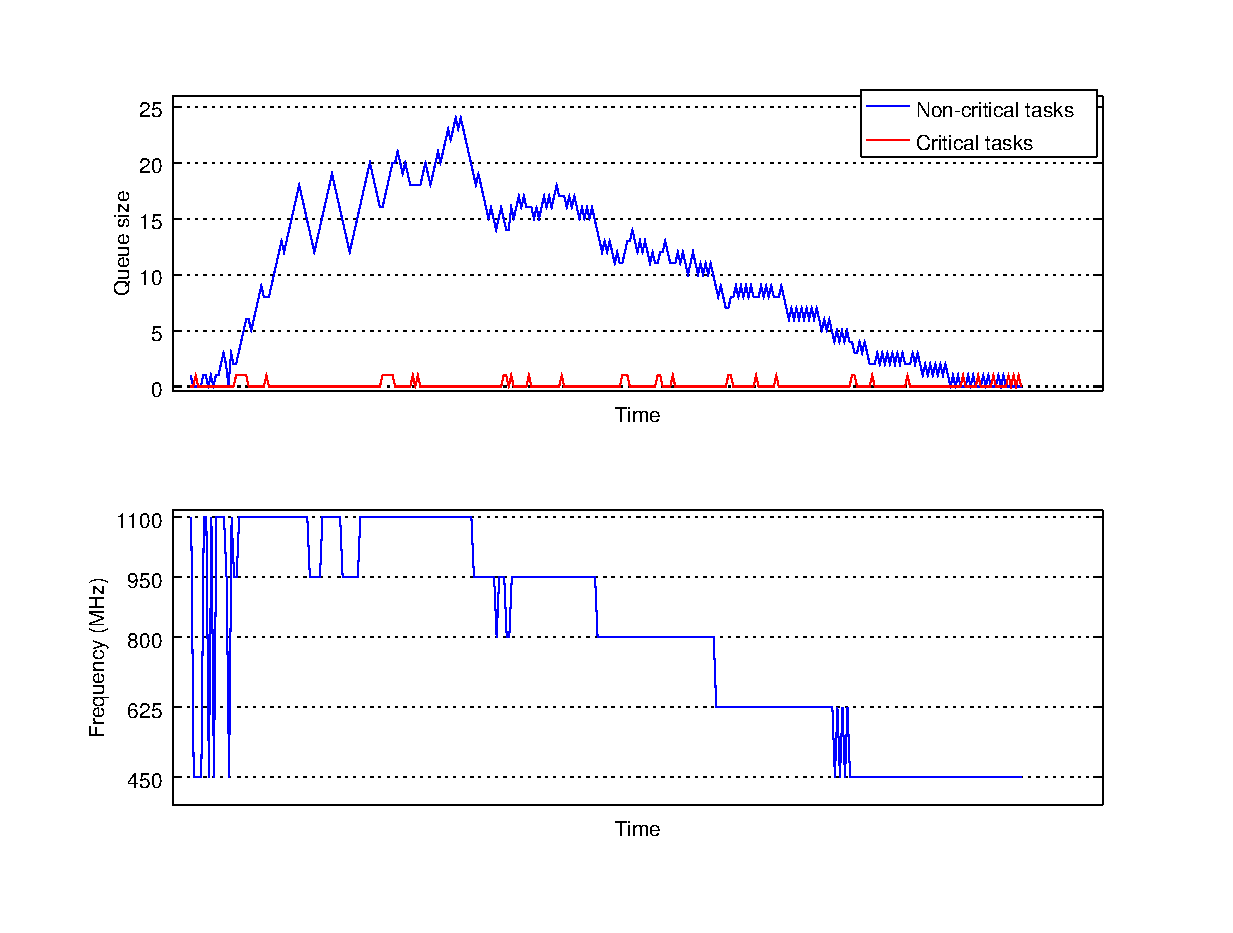
\includegraphics[width=0.9\textwidth]{Plots/politicas/P3_4608-512.eps}
    \vspace{-0.8cm}
    \caption{Política P3: escalado de frecuencia sobre el cluster
      big. Factorización de Cholesky con $m=4608$ y $b=512$, sobre la
      plataforma {\sc Juno}.}
  \end{figure}
\end{frame}

\begin{frame}[shrink]
  \frametitle{Resultados (I)}
  \begin{figure}
    \centering
    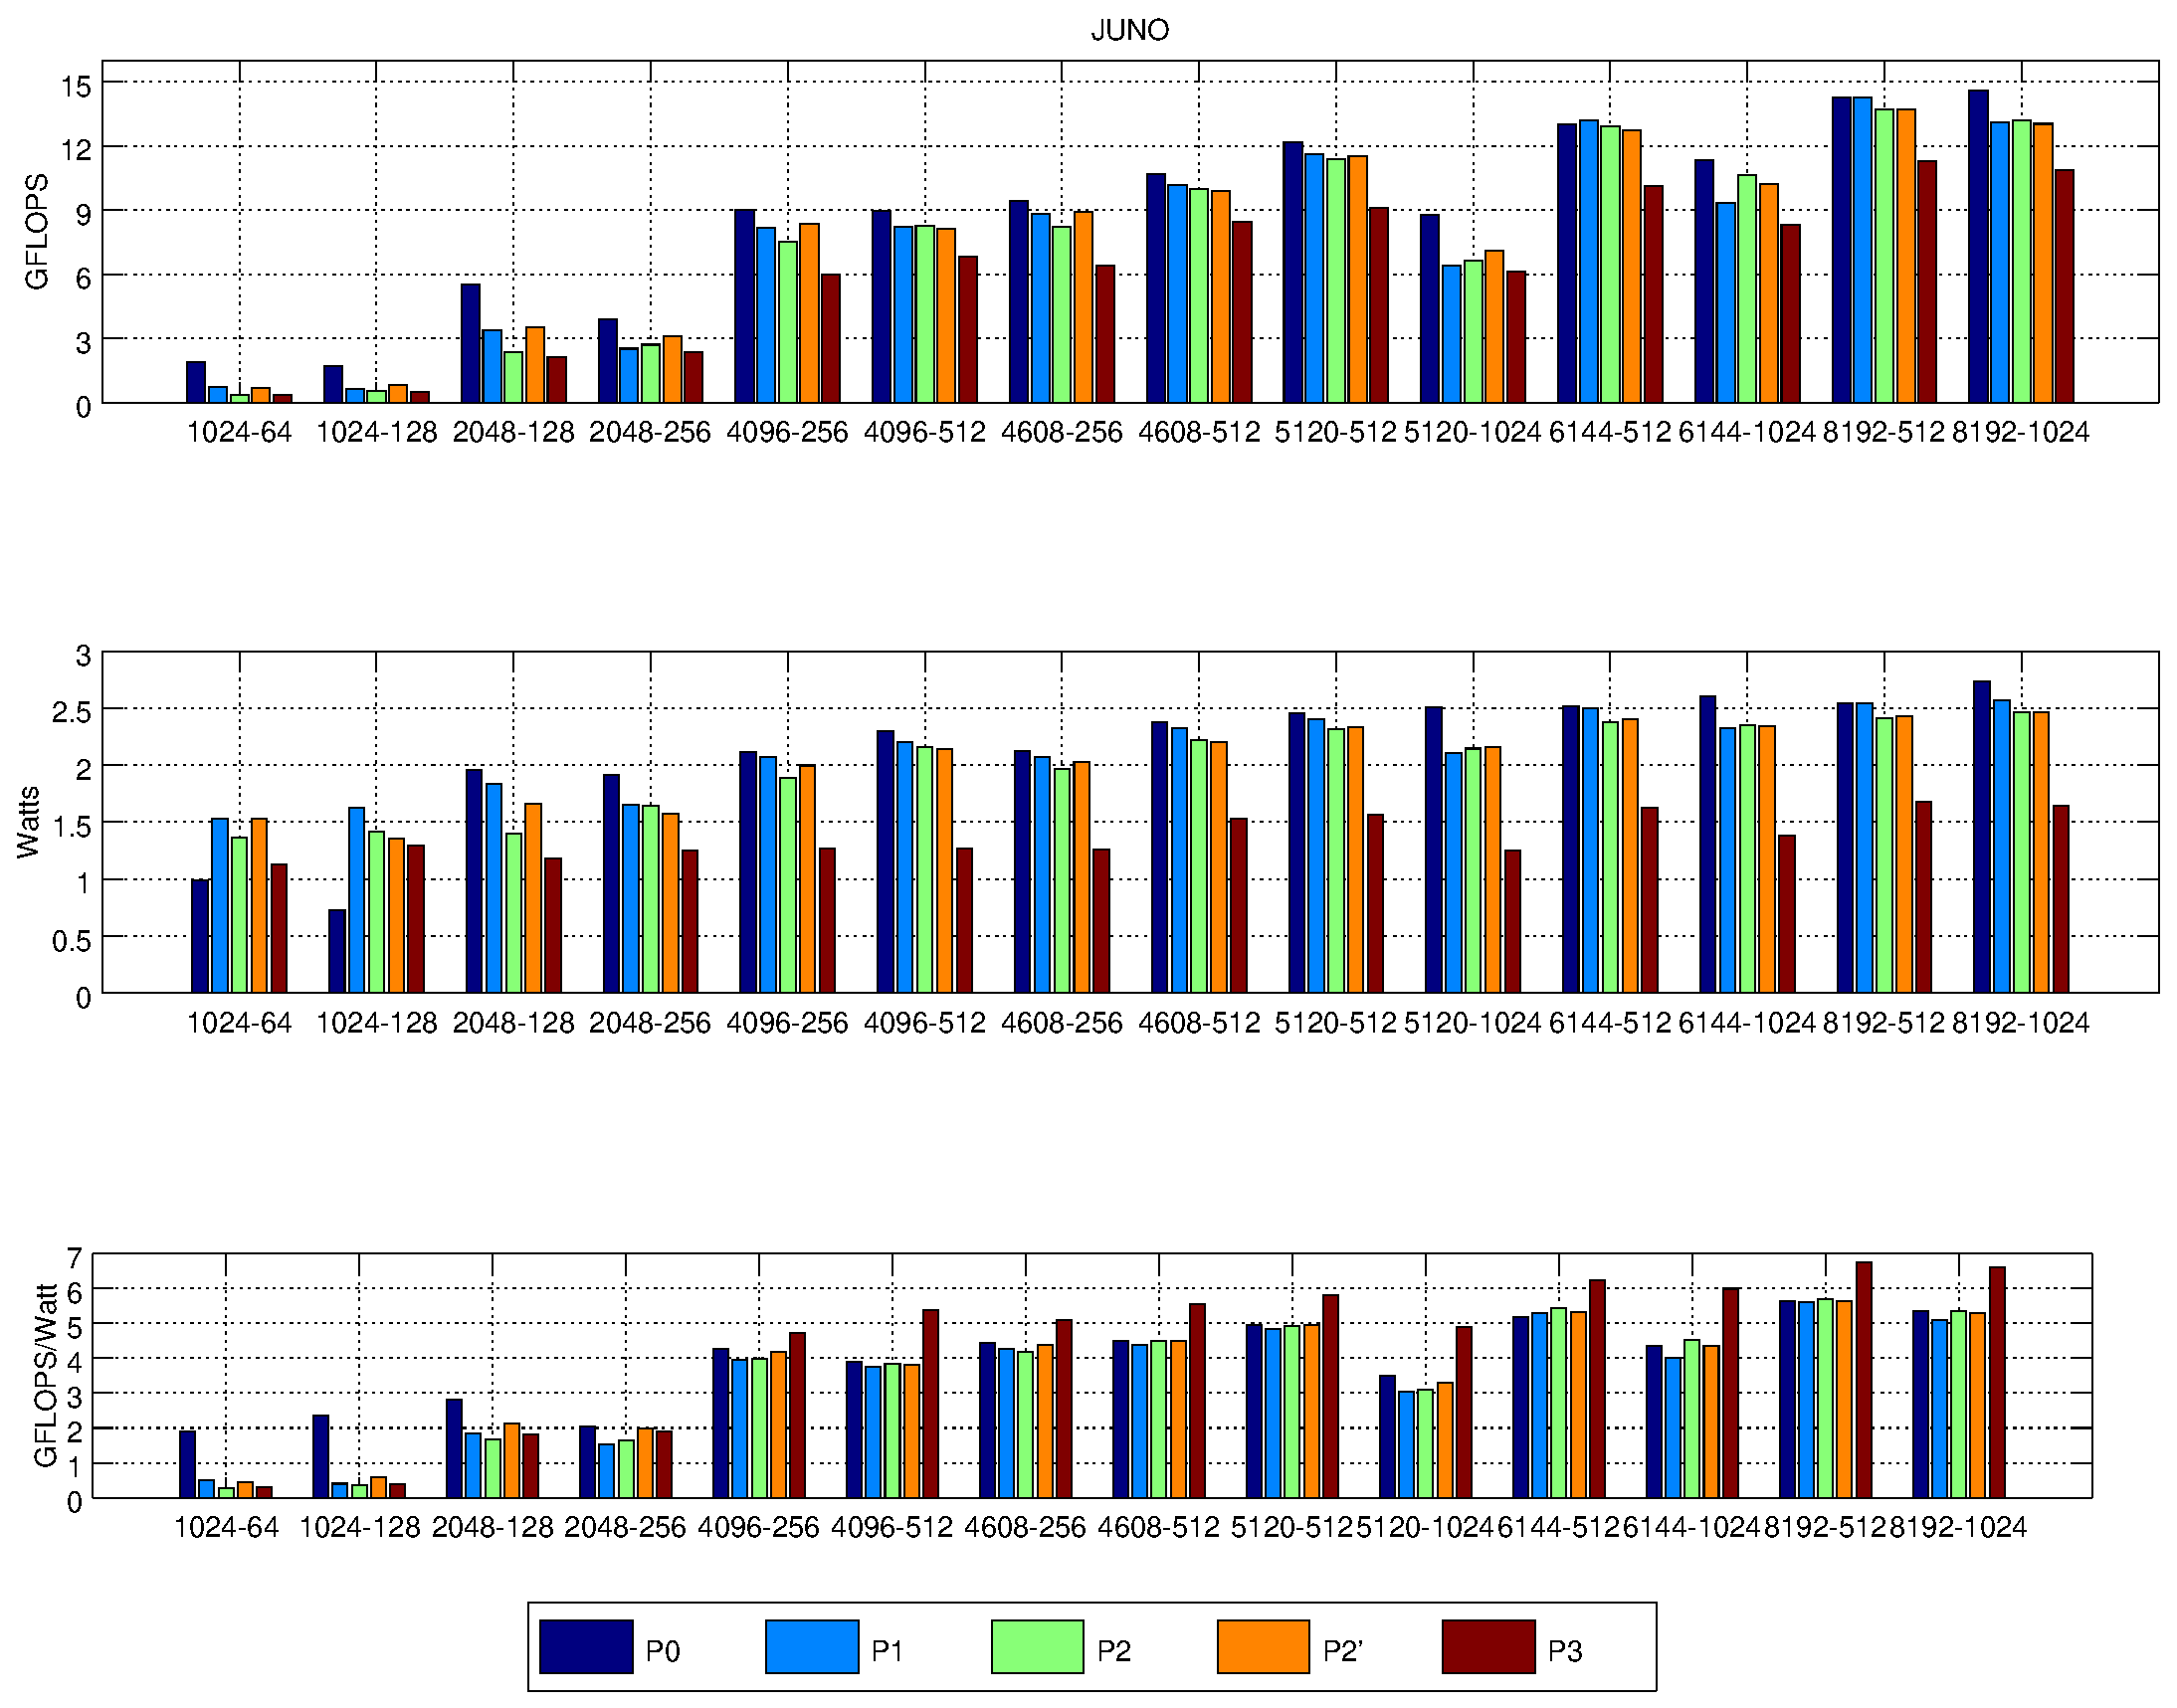
\includegraphics[width=0.9\textwidth]{Plots/dvfs_results/0-4_all_juno.eps}
  \end{figure}
\end{frame}

\begin{frame}
  \frametitle{Resultados (II)}
  \begin{figure}
    \centering
    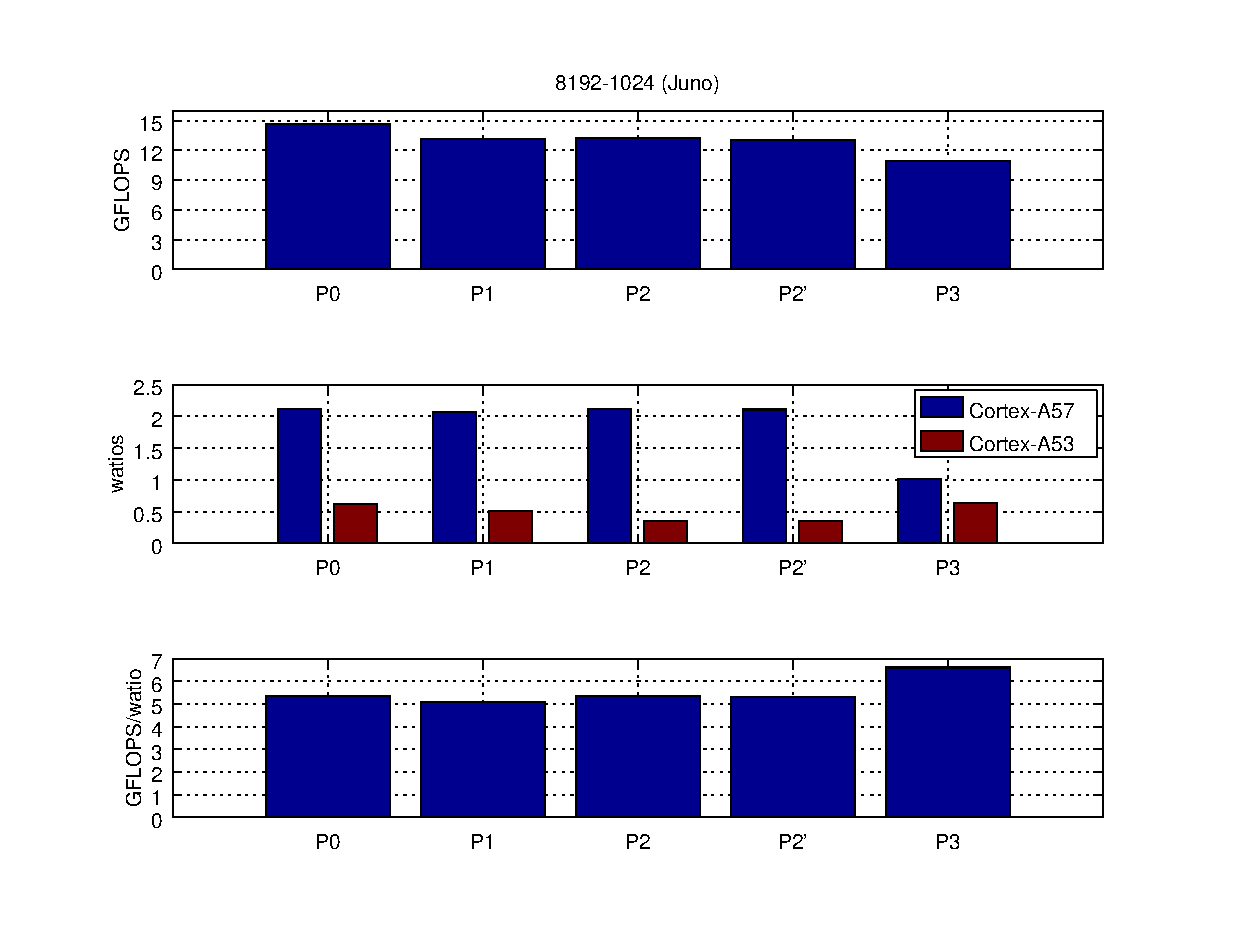
\includegraphics[width=0.8\textwidth]{Plots/dvfs_results/8192-124_0-4_juno.eps}
    \caption{Resultados detallados para las políticas P1-P3 sobre la
      plataforma {\sc Juno} para una factorización de Cholesky con
      $m=8192$ y $b=1024$.}
  \end{figure}
\end{frame}


\begin{frame}
  \frametitle{Técnicas de planificación}
  {\bf Políticas P4 y P5:} Inhabilitación del cluster según la carga de
  trabajo
  \vfill
  \begin{figure}
    \centering
\includegraphics[width=1\textwidth]{Figures/Apagado_tareas.png}\\
    \vspace{1cm}
    \includegraphics[width=1\textwidth]{Figures/Apagado_colas.png}
    \caption{Asignación de tareas para la política P4 sobre una
      factorización de Cholesky con $m=4096$, $b=512$ sobre {\sc Juno}.}
  \end{figure}
\end{frame}


\begin{frame}
  \frametitle{Técnicas de planificación}
  {\bf Política P6:} Desactivación de núcleos en función de la carga de
  trabajo
  \vfill
  \begin{figure}
    \centering
    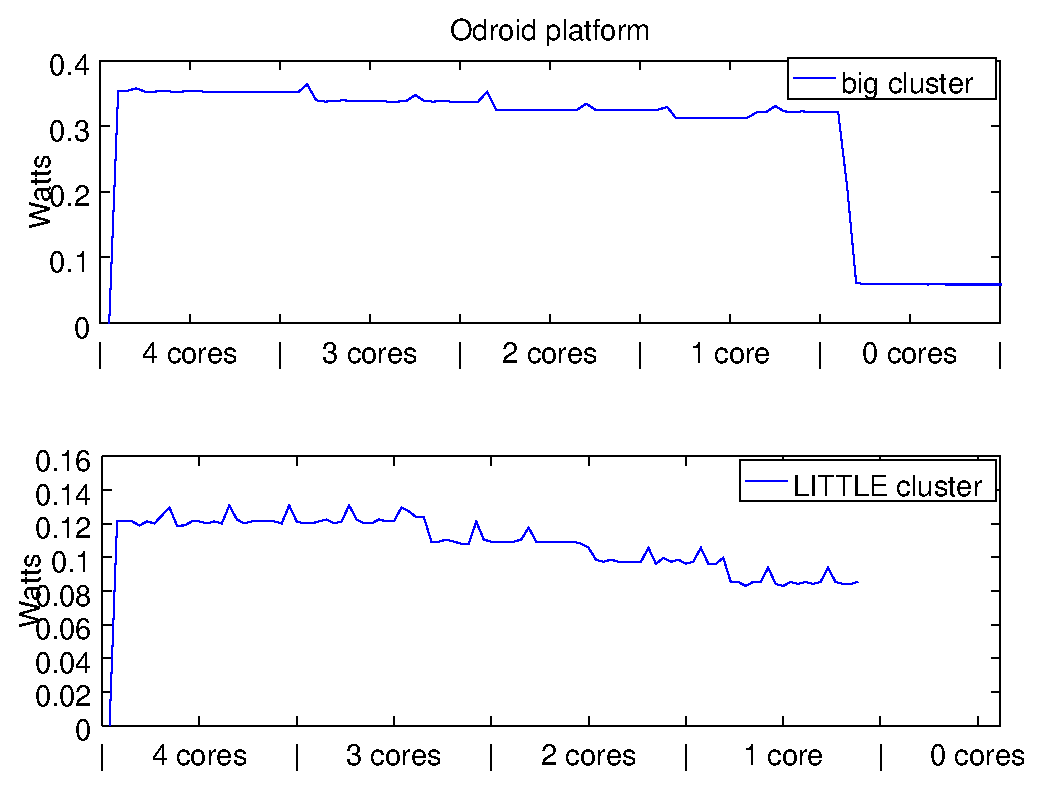
\includegraphics[width=0.8\textwidth]{Plots/modelo_consumo/apagadoOdroid.eps}
    \caption{Consumo energético en función del número de núcleos activos en
      el sistema.}
  \end{figure}
\end{frame}


\begin{frame}
  \frametitle{Resultados (III)}
  {\bf P4 - {\sc Juno}}
  \begin{figure}
    \centering
    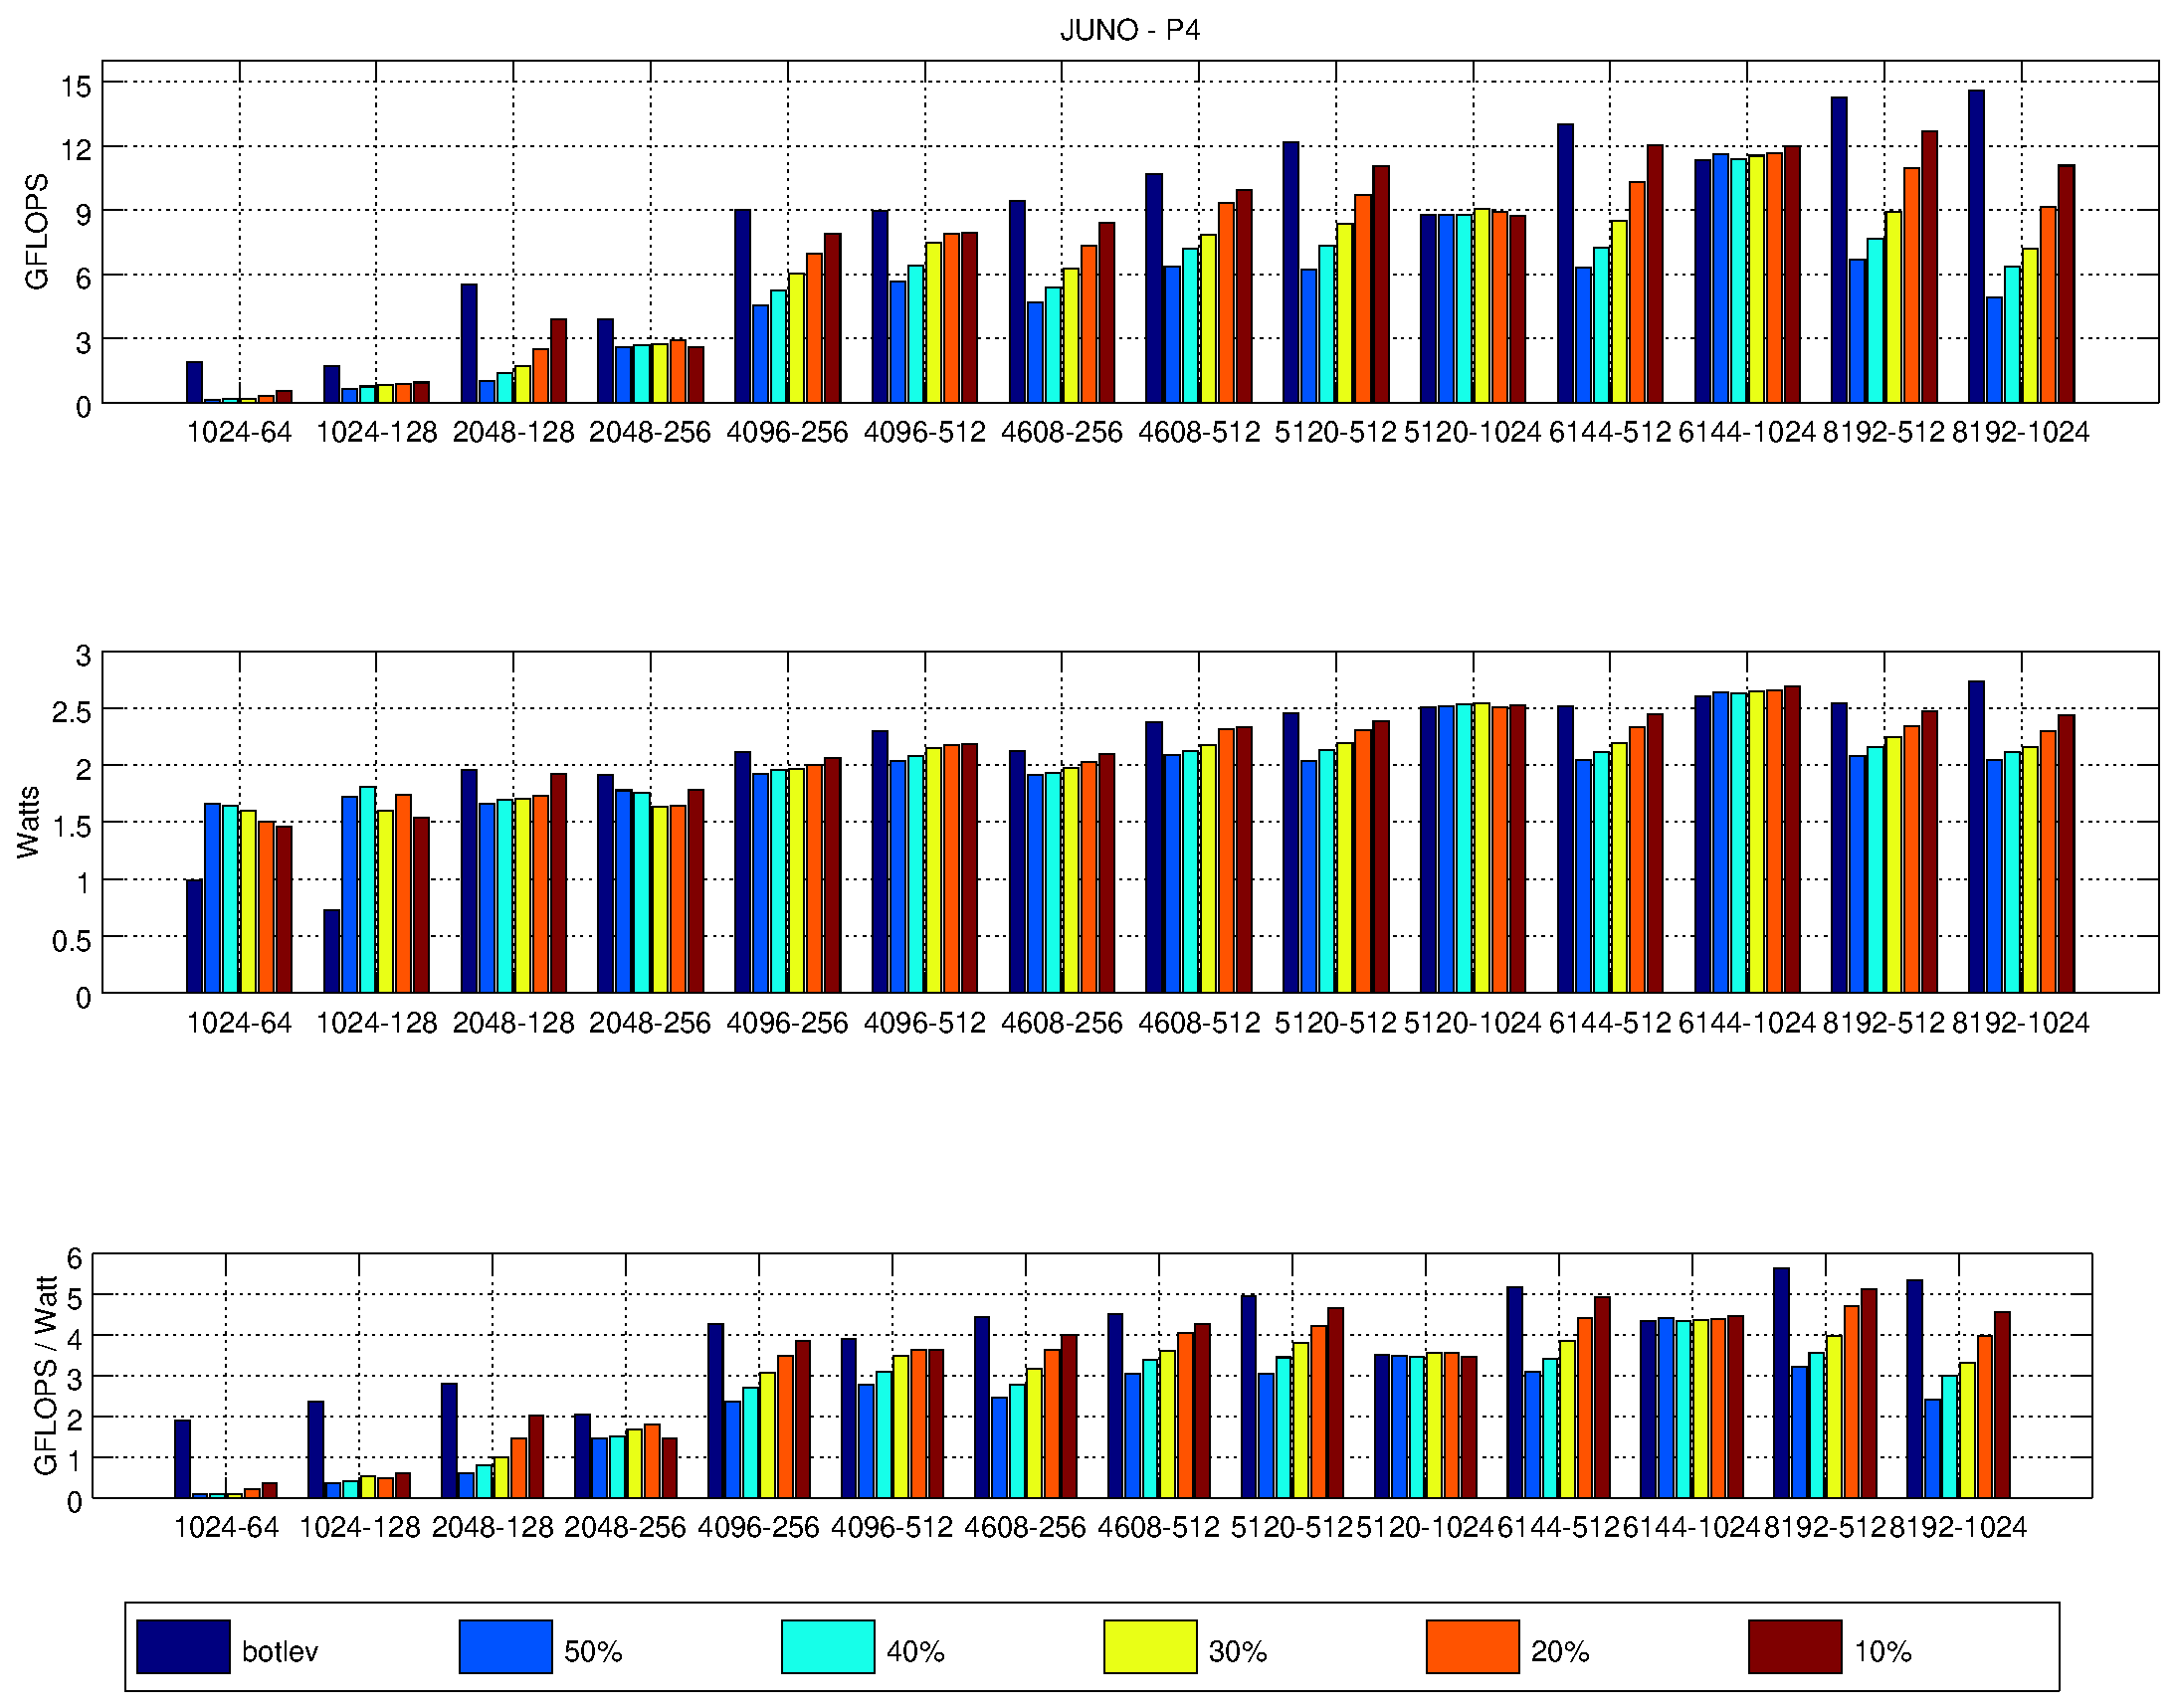
\includegraphics[width=0.9\textwidth]{Plots/sched_results/P4_juno.eps}
  \end{figure}
\end{frame}

\begin{frame}
  \frametitle{Resultados (IV)}
  {\bf P5 - {\sc Juno}}
  \begin{figure}
    \centering
    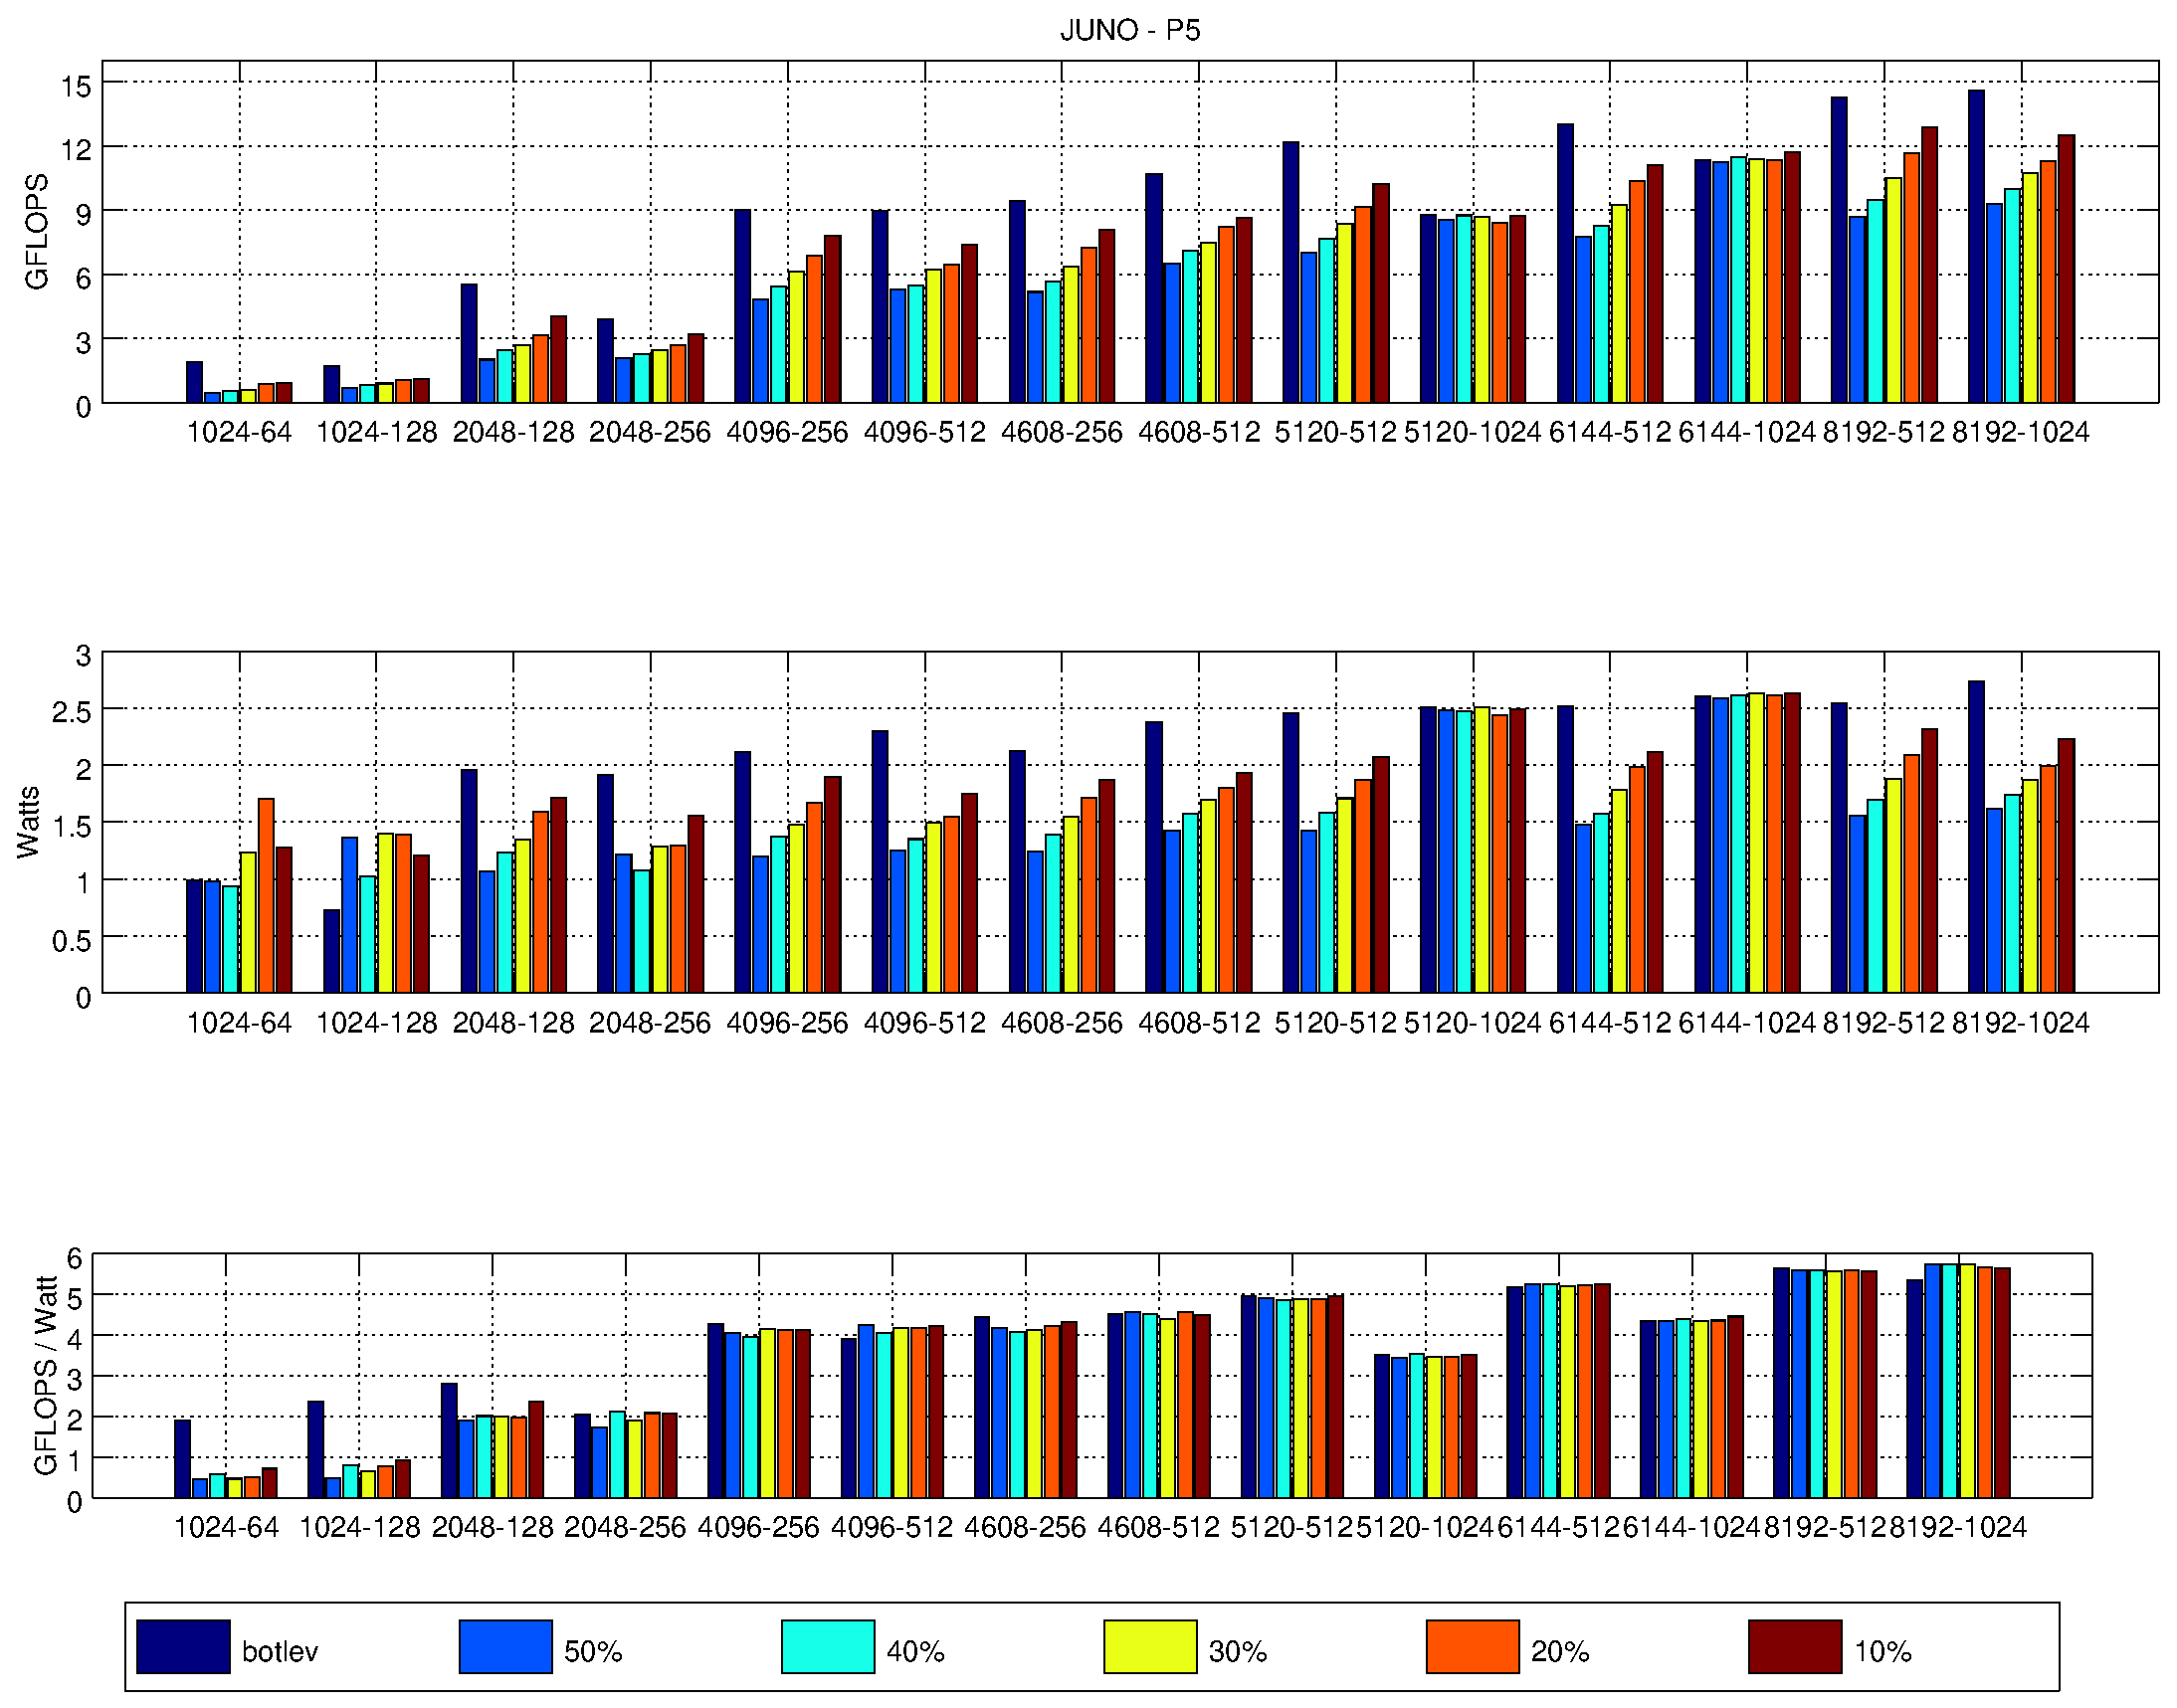
\includegraphics[width=0.9\textwidth]{Plots/sched_results/P5_juno.eps}
  \end{figure}
\end{frame}


\begin{frame}
  \frametitle{Resultados (V)}
  {\bf P6 - {\sc Odroid}}
  \begin{figure}
    \centering
    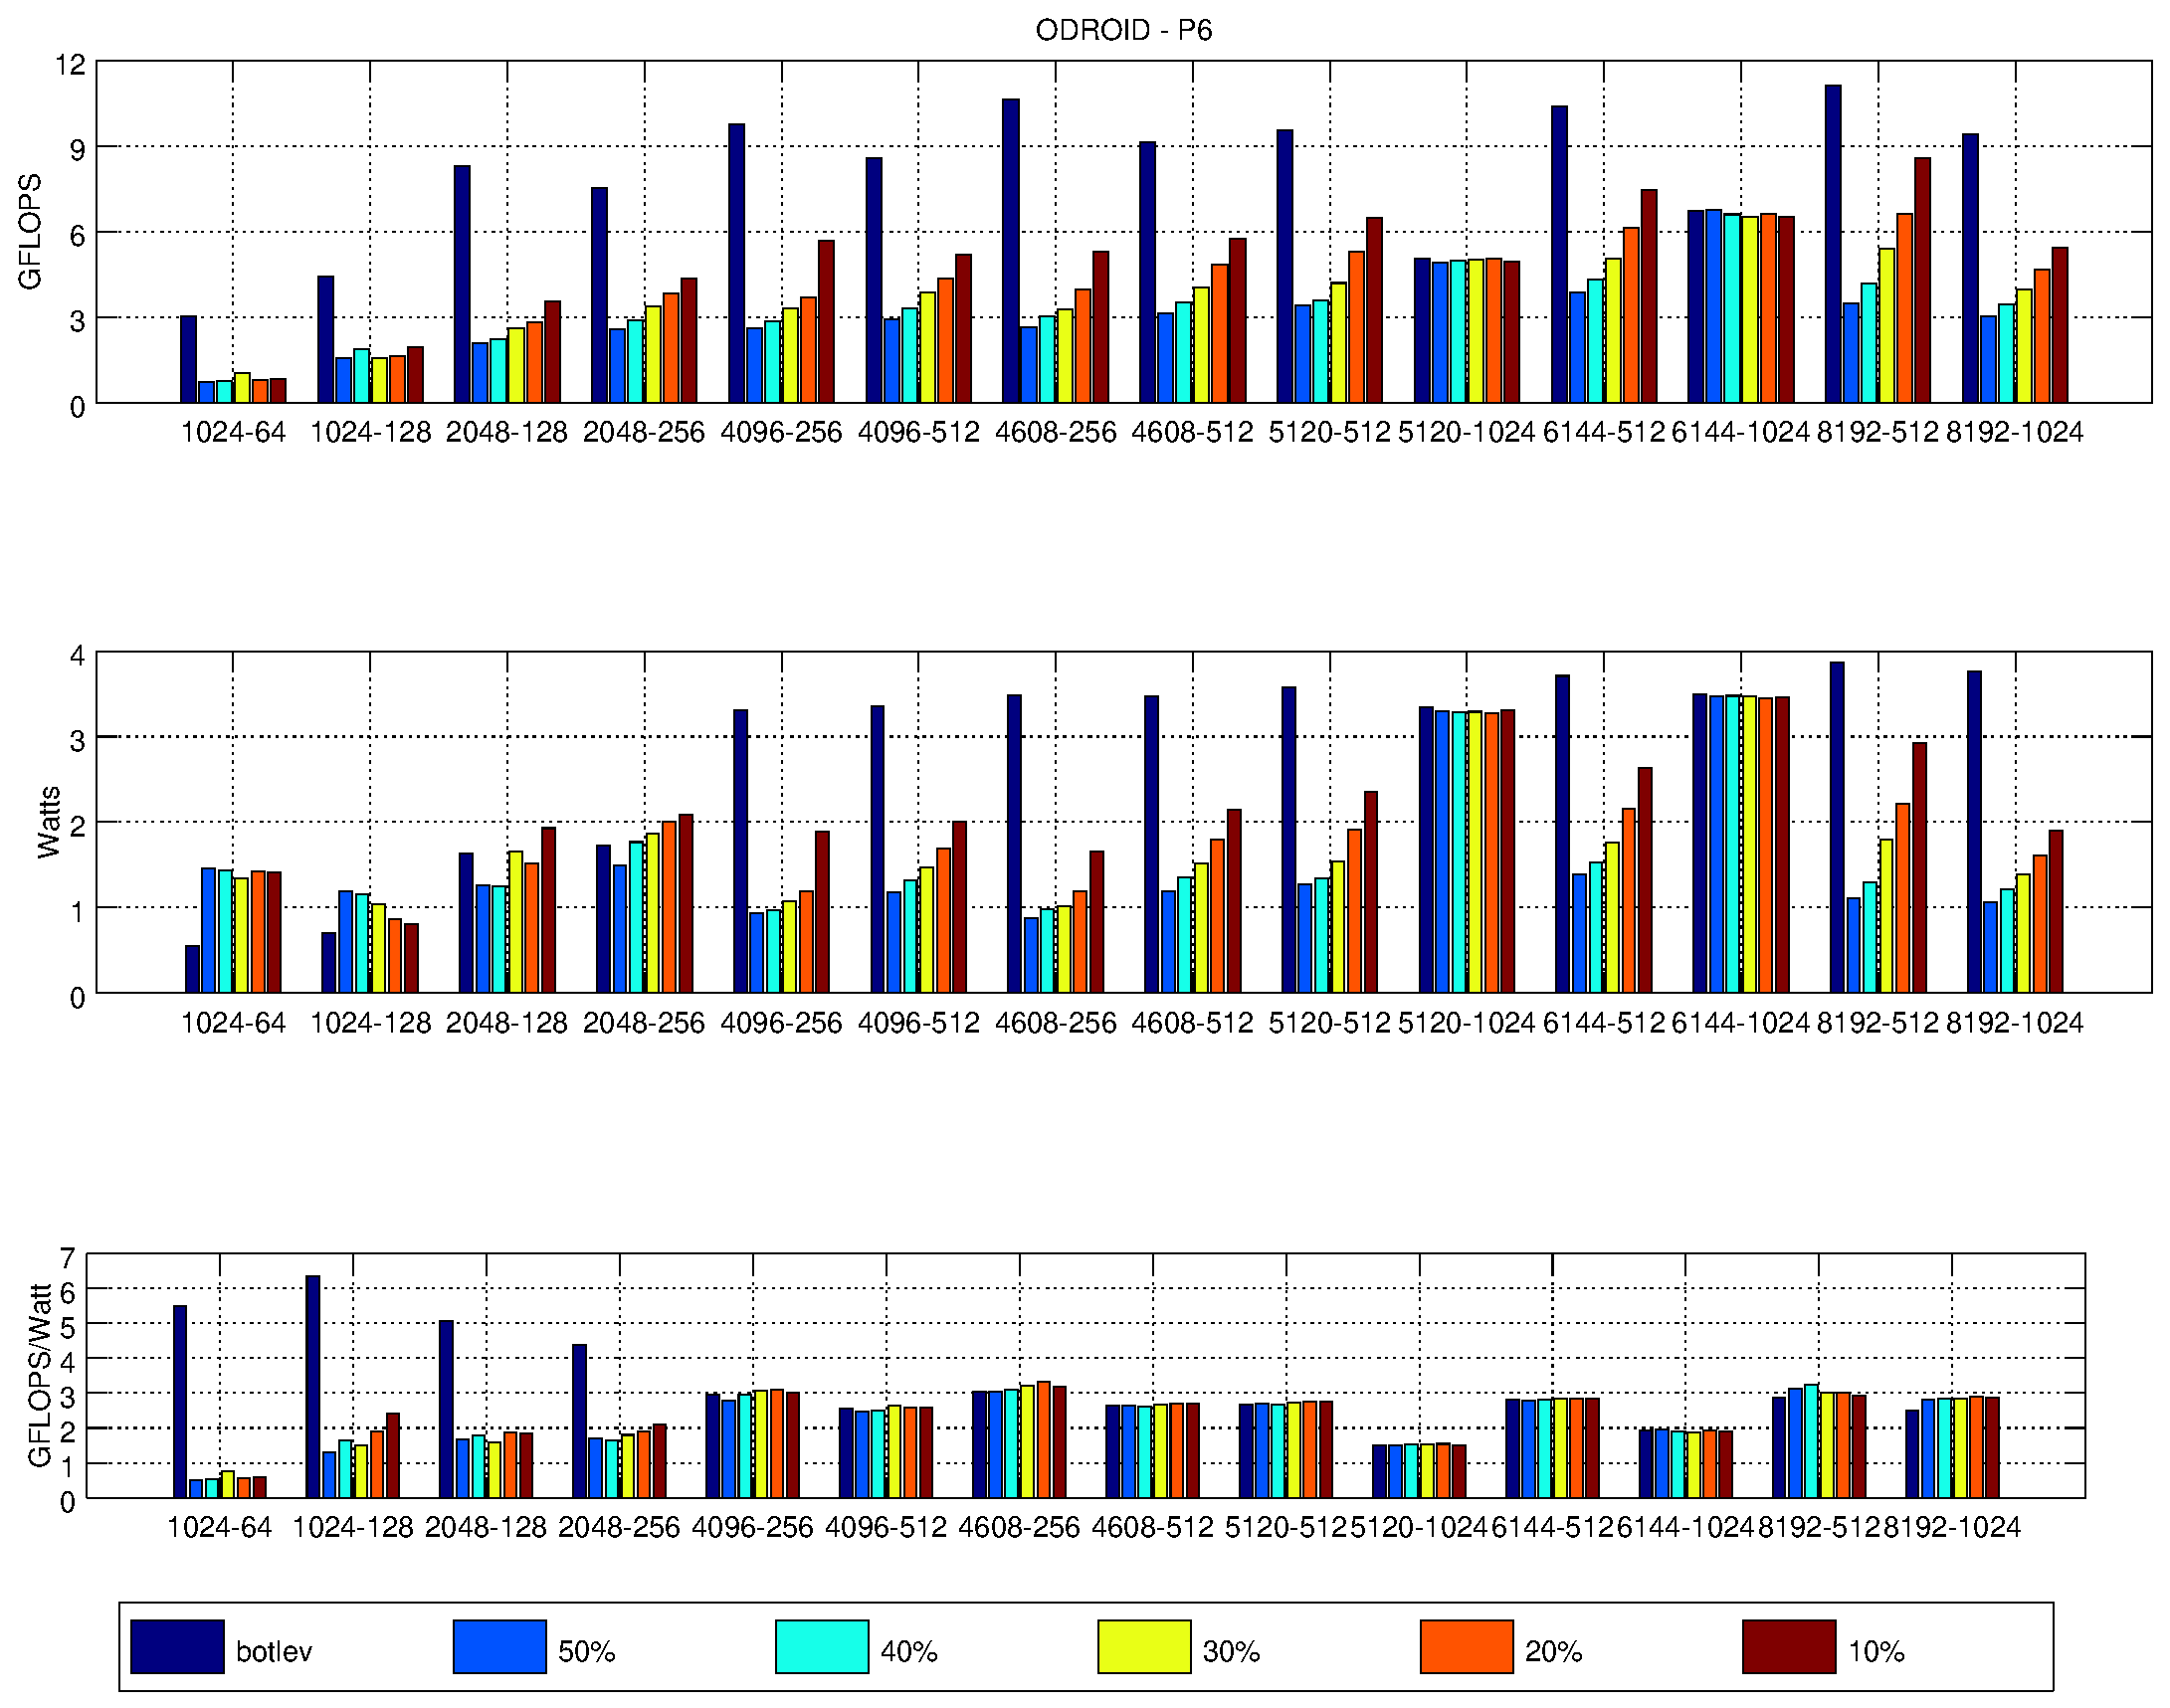
\includegraphics[width=0.9\textwidth]{Plots/sched_results/P6_odroid.eps}
  \end{figure}
\end{frame}
%===========================================================================
\section{Conclusions and future work}
\begin{frame}
  \frametitle{Conclusions and future work}
  {\bf Conclusions:}
  \begin{itemize}
  \item We have explored different techniques to exploit parallelism on
    asymmetric architectures.
    \vfill
  \item To exploit performance:
    \begin{itemize}
    \item We have compared the use of asymmetric libraries + conventional
      runtimes vs specific ad-hoc asymmetry-aware schedulers.
    \item These results have been published in AsHES WorkShop 2016.
    \end{itemize}
  \item To obtain efficient energy executions:
    \begin{itemize}
    \item We have developed frequency scaling techniques over OmpSs
      runtime.
    \item Also, we have modified botlev scheduler to add new scheduling
      policies.
    \end{itemize}
  \end{itemize}

  {\bf Future work:}
  \begin{itemize}
  \item Exploit new grades of asymmetry (not only 4vs4 cores, or 4vs2
    cores).
  \item Study the energy impact of asymmetry-aware libraries.
  \end{itemize}
\end{frame}

%===========================================================================
\begin{frame}
  \begin{center}
    {\huge\bf Muchas gracias}\\[1cm]
    {\Large \em ¿Dudas?}
  \end{center}
\end{frame}


\frame[plain]{\vspace{0.6cm} \centering
  \hspace{0.1cm}
  \begin{minipage}{0.85\textwidth}
    \centering
    \small \textsc{Máster en Ingeniería Informática}\\ \medskip
    \small \textsc{Trabajo fin de Máster} \\ \medskip
    \scriptsize \textsc{20 de septiembre de 2016}
  \end{minipage}\\[0.70cm]
  \small
  \scriptsize
  \titlepage
}
\end{document}
